\documentclass[aspectratio=169,]{beamer}

% -------------------------------------------------------------------------
% 1. REQUIRED PACKAGES (The "Batteries" Quarto usually includes)
% -------------------------------------------------------------------------
\usepackage{graphicx}
\usepackage{booktabs}
\usepackage{longtable}
\usepackage{hyperref}
\usepackage{array}      % <--- ADD THIS LINE HERE
\usepackage[most]{tcolorbox} % REQUIRED for Quarto Callouts
\usepackage{fontawesome5}    % REQUIRED for Callout Icons
\usepackage{framed}          % REQUIRED for standard blocks
\usepackage{tikz}
\usetikzlibrary{arrows.meta}

% Fix for Pandoc's "tightlist"
\providecommand{\tightlist}{%
  \setlength{\itemsep}{0pt}\setlength{\parskip}{0pt}}

% -------------------------------------------------------------------------
% 2. CUSTOM DESIGN PACKAGES
% -------------------------------------------------------------------------
\usepackage{tikz}
\usepackage{calc}
\usepackage{xcolor}
\usepackage{xparse} 
\usepackage{etoolbox} 
\usepackage[default]{sourcesanspro} 
\usetikzlibrary{calc, positioning, shapes.geometric}

% -------------------------------------------------------------------------
% DEFINE QUARTO CALLOUT COLORS (REQUIRED)
% -------------------------------------------------------------------------
% We map these to your "Elegant Dark Mode" aesthetic.
% Note: Quarto expects these EXACT names.

% 1. Note (Blue)
\definecolor{quarto-callout-note-color}{HTML}{3498DB}        % Icon/Title Color
\definecolor{quarto-callout-note-color-frame}{HTML}{2980B9}  % Border Color

% 2. Tip (Green)
\definecolor{quarto-callout-tip-color}{HTML}{27AE60}
\definecolor{quarto-callout-tip-color-frame}{HTML}{2ECC71}

% 3. Important (Red/Crimson)
\definecolor{quarto-callout-important-color}{HTML}{C0392B}
\definecolor{quarto-callout-important-color-frame}{HTML}{E74C3C}

% 4. Warning (Orange)
\definecolor{quarto-callout-warning-color}{HTML}{F39C12}
\definecolor{quarto-callout-warning-color-frame}{HTML}{E67E22}

% 5. Caution (Yellow/Gold)
\definecolor{quarto-callout-caution-color}{HTML}{F1C40F}
\definecolor{quarto-callout-caution-color-frame}{HTML}{D4AC0D}

% Add this right before \begin{document}
\newcommand{\Est}[1]{\textcolor{quarto-callout-important-color}{\mathbf{#1}}}

\providecommand{\estc}[1]{\textcolor[HTML]{1B7837}{#1}}
\makeatletter
\@ifpackageloaded{caption}{}{\usepackage{caption}}
\AtBeginDocument{%
\ifdefined\contentsname
  \renewcommand*\contentsname{Table of contents}
\else
  \newcommand\contentsname{Table of contents}
\fi
\ifdefined\listfigurename
  \renewcommand*\listfigurename{List of Figures}
\else
  \newcommand\listfigurename{List of Figures}
\fi
\ifdefined\listtablename
  \renewcommand*\listtablename{List of Tables}
\else
  \newcommand\listtablename{List of Tables}
\fi
\ifdefined\figurename
  \renewcommand*\figurename{Figure}
\else
  \newcommand\figurename{Figure}
\fi
\ifdefined\tablename
  \renewcommand*\tablename{Table}
\else
  \newcommand\tablename{Table}
\fi
}
\@ifpackageloaded{float}{}{\usepackage{float}}
\floatstyle{ruled}
\@ifundefined{c@chapter}{\newfloat{codelisting}{h}{lop}}{\newfloat{codelisting}{h}{lop}[chapter]}
\floatname{codelisting}{Listing}
\newcommand*\listoflistings{\listof{codelisting}{List of Listings}}
\makeatother
\makeatletter
\makeatother
\makeatletter
\@ifpackageloaded{caption}{}{\usepackage{caption}}
\@ifpackageloaded{subcaption}{}{\usepackage{subcaption}}
\makeatother

% -------------------------------------------------------------------------
% NEW: COLOR THEME COMMANDS (Robust Single-Slide Overrides)
% -------------------------------------------------------------------------

% 1. Light Mode Command
\newcommand{\LightMode}{
  % 1. Draw White Background (TikZ Overlay)
  \begin{tikzpicture}[remember picture, overlay]
    \fill[white] (current page.south west) rectangle (current page.north east);
  \end{tikzpicture}
  % 2. Force Text Colors to Black
  \setbeamercolor{normal text}{fg=black}
  \setbeamercolor{frametitle}{fg=black}
  \setbeamercolor{itemize item}{fg=black}
  \setbeamercolor{structure}{fg=black}
  \usebeamercolor[fg]{normal text}
}

% 2. Black Mode Command
\newcommand{\BlackMode}{
  \begin{tikzpicture}[remember picture, overlay]
    \fill[black] (current page.south west) rectangle (current page.north east);
  \end{tikzpicture}
  \setbeamercolor{normal text}{fg=white}
  \setbeamercolor{frametitle}{fg=white}
  \setbeamercolor{itemize item}{fg=white}
  \setbeamercolor{structure}{fg=white}
  \usebeamercolor[fg]{normal text}
}

% 3. Brand Mode Command
\newcommand{\BrandMode}{
  \begin{tikzpicture}[remember picture, overlay]
    \definecolor{tempBrand}{HTML}{7D181E}
    \fill[tempBrand] (current page.south west) rectangle (current page.north east);
  \end{tikzpicture}
  \setbeamercolor{normal text}{fg=white}
  \setbeamercolor{frametitle}{fg=white}
  \setbeamercolor{itemize item}{fg=white}
  \setbeamercolor{structure}{fg=white}
  \usebeamercolor[fg]{normal text}
}

% -------------------------------------------------------------------------
% 4. UC BERKELEY THEME (Modern Matte) - FIXED SCOPE
% -------------------------------------------------------------------------

% 1. DEFINE COLORS GLOBALLY (Required for assumptionbox and modes)
\definecolor{BerkeleyBlue}{HTML}{003262}
\definecolor{CaliforniaGold}{HTML}{FDB515}
\definecolor{BerkeleyMatte}{HTML}{0D2D52} 
\definecolor{SoftWhite}{HTML}{F8F9FA}

% 4. UC Berkeley Theme (Modern Matte)
\newcommand{\BerkeleyMode}{
  % 2. Draw Background AND Title
  \begin{tikzpicture}[remember picture, overlay]
    % Background Fill (Covers old title)
    \fill[BerkeleyMatte] (current page.south west) rectangle (current page.north east);
    % Gold Accent Strip
    \fill[CaliforniaGold] (current page.south west) rectangle ($(current page.north west)+(0.15cm,0)$);
    % REDRAW TITLE ON TOP
    \node[anchor=west, white, font=\Large\bfseries] at ($(current page.north west)+(1cm,-1cm)$) {\insertframetitle};
  \end{tikzpicture}
  
  % 3. Set Text Colors
  \setbeamercolor{normal text}{fg=SoftWhite}
  \setbeamercolor{frametitle}{fg=BerkeleyMatte} % Hide original title
  \setbeamercolor{itemize item}{fg=CaliforniaGold} 
  \setbeamercolor{structure}{fg=CaliforniaGold}
  
  \usebeamercolor[fg]{normal text}
}

% 5. UC Berkeley Theme (Academic Light)
\newcommand{\BerkeleyLightMode}{
  % (Color definitions removed here as they are now global)
  
  % 2. Draw Background AND Title
  \begin{tikzpicture}[remember picture, overlay]
    % Background Fill
    \fill[white] (current page.south west) rectangle (current page.north east);
    % Blue Header Bar
    \fill[BerkeleyBlue] (current page.north west) rectangle ($(current page.north east)+(0,-1.4cm)$);
    % Gold Line
    \fill[CaliforniaGold] ($(current page.north west)+(0,-1.4cm)$) rectangle ($(current page.north east)+(0,-1.45cm)$);
    % REDRAW TITLE ON TOP
    \node[anchor=west, white, font=\Large\bfseries] at ($(current page.north west)+(1cm,-0.7cm)$) {\insertframetitle};
  \end{tikzpicture}
  
  % 3. Set Text Colors
  \setbeamercolor{normal text}{fg=black}
  \setbeamercolor{frametitle}{fg=white} 
  \setbeamercolor{itemize item}{fg=BerkeleyBlue}
  \setbeamercolor{structure}{fg=BerkeleyBlue}
  
  \usebeamercolor[fg]{normal text}
}

% -------------------------------------------------------------------------
% NEW: ACADEMIC POWER LAYOUTS
% -------------------------------------------------------------------------

% 1. Statement Layout (Big Impact Transitions)
% Usage: ::: {.layout-statement} Content :::
\newenvironment{layout-statement}{
  \vspace*{\fill}
  \centering
  \Huge \bfseries
  \setbeamercolor{normal text}{fg=CaliforniaGold} % Use Gold for impact
  \usebeamercolor[fg]{normal text}
}{
  \vspace*{\fill}
}

% 2. Dense Data Layout (Regression Tables)
% Usage: ::: {.layout-dense} Table :::
\newenvironment{layout-dense}{
  \vspace*{\fill}
  \tiny                  % Force tiny font
  \setlength\tabcolsep{2pt} % Tighten table columns
  \centering
}{
  \vspace*{\fill}
}

% 3. Split Slide Macro (Vertical Centering)
% Usage: \SplitSlide{Left Content}{Right Content}
\newcommand{\SplitSlide}[2]{
  \begin{columns}[c] % 'c' option forces vertical centering
    \begin{column}{0.48\textwidth}
      #1
    \end{column}
    \begin{column}{0.48\textwidth}
      \centering
      #2
    \end{column}
  \end{columns}
}

% -------------------------------------------------------------------------
% 3. DYNAMIC BACKGROUND & CONTRAST LOGIC
% -------------------------------------------------------------------------
  \definecolor{mainbg}{HTML}{0D2D52}

\setbeamercolor{background canvas}{bg=mainbg}

% Logic to calculate luminance and set text color automatically
\makeatletter
\newcommand{\AutoSetContrast}{
  \extractcolorspec{mainbg}{\mainbgspec}
  \expandafter\convertcolorspec\mainbgspec{rgb}\mainbgrgb
  \def\calculatebrightness##1,##2,##3;{
    \pgfmathparse{0.2126*##1 + 0.7152*##2 + 0.0722*##3}
  }
  \expandafter\calculatebrightness\mainbgrgb;
  \pgfmathparse{\pgfmathresult > 0.5 ? 1 : 0}
  \ifnum\pgfmathresult=1
    \definecolor{maintext}{HTML}{222222}
    \definecolor{dimtext}{HTML}{555555}
  \else
    \definecolor{maintext}{HTML}{FFFFFF}
    \definecolor{dimtext}{HTML}{CCCCCC}
  \fi
}
\makeatother

\AutoSetContrast

\setbeamercolor{normal text}{fg=maintext}
\setbeamercolor{frametitle}{fg=maintext}
\setbeamercolor{title}{fg=maintext}
\setbeamercolor{structure}{fg=maintext} 

% -------------------------------------------------------------------------
% 4. FOOTER CUSTOMIZATION
% -------------------------------------------------------------------------
\setbeamercolor{footline}{fg=dimtext}
\setbeamerfont{footline}{size=\tiny}

\newtoggle{hidesection}
\togglefalse{hidesection}

\setbeamertemplate{footline}{
  \begin{beamercolorbox}[wd=\paperwidth, ht=2.5ex, dp=1.125ex, leftskip=.3cm, rightskip=.3cm]{footline}
    \iftoggle{hidesection}{}{
      \insertsectionhead
    }
    \hfill
    \insertframenumber
  \end{beamercolorbox}
}
\setbeamertemplate{navigation symbols}{}

% -------------------------------------------------------------------------
% 5. CUSTOM COMMANDS & ENVIRONMENTS (FIXED FOR STABILITY)
% -------------------------------------------------------------------------
\NewDocumentCommand{\navbutton}{ O{} O{fill=gray} m }{
  \hyperlink{#1}{
    \tikz[baseline=(node.base)]{
      \node(node)[
        anchor=base,
        rounded corners=3pt,
        inner sep=5pt,
        text=white,
        font=\small\bfseries,
        #2
      ]{#3};
    }
  }
}

\newenvironment{layout-math}{
  \vspace*{\fill}
  \centering
  \begin{minipage}{\linewidth}
  \centering
}{
  \end{minipage}
  \vspace*{\fill}
}

% SAFE Layout for Tables (Removed risky \makebox)
\newenvironment{layout-table}{
  \vspace*{\fill}
  \begin{center}
}{
  \end{center}
  \vspace*{\fill}
}

% SAFE Layout for Full Figures (Uses LRBOX to capture content first)
\newsavebox{\fullfigbox}
\newenvironment{layout-full-figure}{
  \begin{lrbox}{\fullfigbox}
    \begin{minipage}{\paperwidth}
      \centering
}{
    \end{minipage}
  \end{lrbox}
  \begin{tikzpicture}[remember picture, overlay]
    \node[anchor=center, inner sep=0pt] at (current page.center) {
      \usebox{\fullfigbox}
    };
  \end{tikzpicture}
}

\newcommand{\hidefootersection}{\global\toggletrue{hidesection}}
\newcommand{\showfootersection}{\global\togglefalse{hidesection}}


% -------------------------------------------------------------------------
% CUSTOM BERKELEY CALLOUT BOX
% -------------------------------------------------------------------------
\newtcolorbox{assumptionbox}[1]{
  enhanced,
  colback=SoftWhite,       % White-ish background
  colframe=CaliforniaGold, % Gold Border
  coltitle=SoftWhite,      % White Title Text
  colbacktitle=BerkeleyMatte, % Berkeley Blue Title Background
  title={#1},
  fonttitle=\bfseries\small,
  arc=2pt,                 % Slight rounded corners
  boxrule=1pt,             % Thin elegant border
  left=5pt, right=5pt, top=5pt, bottom=5pt, % Padding
  titlerule=0pt,
  width=\linewidth
}

% -------------------------------------------------------------------------
% 6. DOCUMENT BODY
% -------------------------------------------------------------------------
\title{Internalizing Environmental Risk: Insurance Design and Firm
Behavior in Hazardous Industries}
\author{Kaleb K. Javier}

\begin{document}

\frame{\titlepage}

\begin{frame}{}
\phantomsection\label{section}
\LightMode

\begin{columns}[c]
\begin{column}{0.5\textwidth}
\centering
\includegraphics[width=\linewidth,height=0.8\textheight,keepaspectratio]{../../Data/tank_jpg.jpg}
\end{column}
\begin{column}{0.5\textwidth}
\centering
\includegraphics[width=\linewidth,height=0.8\textheight,keepaspectratio]{../../Data/LUST.jpg}
\end{column}
\end{columns}
\end{frame}

\begin{frame}{Compulsory insurance works only if it prices risk}
\phantomsection\label{compulsory-insurance-works-only-if-it-prices-risk}
\BerkeleyLightMode

\begin{itemize}
\tightlist
\item
  U.S. environmental law makes polluters pay for the harm they cause:
  strict liability (OPA 1990, SMCRA 1977, CERCLA 1980, RCRA 1976).
\item
  It also requires proof they can pay: bonding, minimum assets, or
  compulsory insurance.
\item
  When that proof is insurance, how the insurance is priced decides
  whether the firm has any reason to cut risk.
\end{itemize}

\vfill

\centering\textbf{This paper examines the design and efficacy of compulsory liability insurance as a financial responsibility instrument, using underground storage tanks (USTs) as a case study for environmentally hazardous settings.}
\end{frame}

\begin{frame}{(UST) leaks (LUSTs) are common, costly, and borne by
others}
\phantomsection\label{ust-leaks-lusts-are-common-costly-and-borne-by-others}
\BerkeleyLightMode

\begin{itemize}
\tightlist
\item
  About 1 in 4 facilities leaks over a 30-year life, as high as oil and
  gas wells.
\item
  USTs are the top source of US groundwater contamination; petroleum and
  benzene reach drinking-water wells (EPA 2024).
\item
  Cleanups are costly: median about \$136k, mean about \$403k per site
  (my claims data).
\item
  Contamination reaches drinking water and lowers infant birthweight
  (Marcus 2021).
\item
  The public funds most states use to cover cleanups are winding down:
  more than a dozen of the 37 fund states are set to close theirs this
  decade (ASTSWMO State Fund Survey 2025).
\end{itemize}

\vfill

\centering\textit{Leak risk is not random: it rises with tank age and construction, both of which an insurer can observe and price.}
\end{frame}

\begin{frame}{A clean natural experiment: Texas, 1998}
\phantomsection\label{a-clean-natural-experiment-texas-1998}
\BerkeleyLightMode

\begin{itemize}
\tightlist
\item
  Every US gas station stores fuel underground: about 140,000
  facilities, 550,000 tanks (EPA 2024).
\item
  Since 1988, every owner must carry at least \$1M in coverage (RCRA
  Subtitle I).
\item
  Most states use a \textbf{state-run, uniform premium}: everyone pays
  the same regardless of risk, so owners have no reason to retire old
  tanks.
\item
  \textbf{Texas, December 22, 1998:} the fund closed overnight. About
  26,000 facilities moved to \textbf{risk-rated private insurance},
  driven by the fund's insolvency, not by any change in Texas tanks.
\end{itemize}
\end{frame}

\begin{frame}{This work answers 3 questions}
\phantomsection\label{this-work-answers-3-questions}
\BerkeleyLightMode

\textbf{Q1. Observability.} Is release risk predictable from observable
tank characteristics? If not, the premium schedule is noise, not signal.

\vspace{0.2cm}

\textbf{Q2. Behavior.} Does risk-based pricing change closure,
replacement, and release outcomes?

\vspace{0.2cm}

\textbf{Q3. Welfare.} How much of the first-best welfare gain does
risk-rated pricing capture?

\vfill

\centering\textit{Three answers, one argument: risk is priceable (Q1), so pricing it moves behavior (Q2), and that behavior change recovers part, not all, of the lost welfare (Q3).}
\end{frame}

\begin{frame}{What am are doing this summer at PERC}
\phantomsection\label{what-am-are-doing-this-summer-at-perc}
\BerkeleyLightMode

\textbf{1. Who responds, and what it does to local markets (reduced form).}

\begin{itemize}
\tightlist
\item
  Heterogeneity by geography (urban vs rural) and firm type (branded vs
  independent): which firms exit, which replace
\item
  Whether the reform raised or lowered local market concentration
\end{itemize}

\vspace{0.25cm}

\textbf{2. Cross-subsidies under the uniform premium (reduced form).}

\begin{itemize}
\tightlist
\item
  Use the claims data to estimate each facility's actuarially fair
  premium, then compare it to what it pays
\item
  Measure how much low-risk facilities subsidize high-risk ones under a
  uniform premium
\end{itemize}

\vspace{0.25cm}

\textbf{3. The structural model.}

\begin{itemize}
\tightlist
\item
  Estimate the portfolio model, then run the four counterfactuals and
  deliver the welfare comparison
\end{itemize}
\end{frame}

\begin{frame}{More Details}
\phantomsection\label{more-details}
\BerkeleyLightMode

\hypertarget{slide-roadmap}{}

\vspace{0.2cm}

\begin{center}
\large
\renewcommand{\arraystretch}{1.7}
\begin{tabular}{ll}
\textbf{Section} & \textbf{Jump to} \\
\hline
Data                  & \navbutton[slide-data][fill=BerkeleyBlue, font=\small, inner sep=4pt]{Data $\rightarrow$} \\[4pt]
Empirical Approach    & \navbutton[slide-rf][fill=BerkeleyBlue, font=\small, inner sep=4pt]{Empirical Approach $\rightarrow$} \\[4pt]
Results               & \navbutton[slide-results][fill=BerkeleyBlue, font=\small, inner sep=4pt]{Results $\rightarrow$} \\[4pt]
Structural Model      & \navbutton[slide-structural][fill=BerkeleyBlue, font=\small, inner sep=4pt]{Structural Model $\rightarrow$} \\
\hline
\end{tabular}
\end{center}
\end{frame}

\begin{frame}{}
\phantomsection\label{section-1}
\BerkeleyMode

\hypertarget{slide-data}{}

\begin{center}
\Huge \textbf{Data}
\end{center}

\begin{tikzpicture}[remember picture, overlay]
\node[anchor=south east, inner sep=0pt] at ([xshift=-10pt, yshift=10pt]current page.south east) {%
  \navbutton[slide-roadmap][fill=BerkeleyBlue!60, font=\tiny, inner sep=2pt]{$\leftarrow$ Roadmap}%
};
\end{tikzpicture}
\end{frame}

\begin{frame}{Data: three collection efforts, 18 usable states}
\phantomsection\label{data-three-collection-efforts-18-usable-states}
\BerkeleyLightMode

\begin{itemize}
  \item \textbf{State + EPA administrative records} --- UST inventory and confirmed releases from all 50 states and EPA LUST Finder; tank-level attributes (install date, wall type, piping, leak detection) and cleanup dispositions
  \hfill \navbutton[baseline-table][fill=BerkeleyBlue, font=\tiny, inner sep=2pt]{Summary statistics $\rightarrow$}

  \vspace{0.25cm}

  \item \textbf{Cleanup cost data} --- Trust-fund claims from 6 control states; first multistate per-site cleanup cost study; median \$136k, mean \$403k; right tail dominates expected loss
  \hfill \navbutton[cost-dist-pooled][fill=BerkeleyBlue, font=\tiny, inner sep=2pt]{Claims distribution $\rightarrow$}

  \vspace{0.25cm}

  \item \textbf{TX insurance rate filings} --- Mid-Continent Casualty SERFF filings, 2006--2024; reconstructs the risk-based premium schedule $P(s)$ at the tank level from base rates, ILFs, and attribute credits/debits
  \hfill \navbutton[premium-divergence][fill=BerkeleyBlue, font=\tiny, inner sep=2pt]{Premium figure $\rightarrow$}
\end{itemize}

\vspace{0.2cm}

\textbf{Why 18 states?} 20 of 38 flat-fee states dropped: missing
closure dates, install dates, or wall construction variables. The 17
controls plus Texas have complete records across all three dimensions.
\end{frame}

\begin{frame}
\LightMode

\hypertarget{baseline-table}{}
\vspace{0.1cm}
\begin{center}
\footnotesize
\setlength{\tabcolsep}{5pt}
\renewcommand{\arraystretch}{1.08}
\begin{tabular}{l rr rr cc}
\hline
 & \multicolumn{2}{c}{\textbf{Alive-at-reform}} & \multicolumn{2}{c}{\textbf{Matched (birth-CEM)}} & \multicolumn{2}{c}{\textbf{SMD}} \\
\cline{2-3}\cline{4-5}\cline{6-7}
 & Texas & Control & Texas & Control & Before & After \\
\hline
Facilities & 54,379 & 198,291 & 18,914 & 86,331 &  &  \\
Tanks at reform & 60,651 & 269,660 & 52,173 & 235,423 &  &  \\
Share single-walled & 89\% & 89\% & 89\% & 89\% & -0.011 & -0.001 \\
Share pre-1989 vintage & 75\% & 68\% & 75\% & 72\% & +0.157 & +0.071 \\
Mean tank age at reform & 15.4 & 16.8 & 15.3 & 15.2 & -0.117 & +0.015 \\
Tanks per facility (med [IQR]) & 3 [2-3] & 2 [1-3] & 3 [2-3] & 3 [2-4] &  &  \\
Total capacity, k gal (med [IQR]) & 18 [8-29] & 13 [3-25] & 22 [14-30] & 16 [4-28] &  &  \\
Mean facility tank age & 16.1 & 20.1 & 17.4 & 18.9 & -0.264 & -0.091 \\
\hline
\end{tabular}
\end{center}


\vspace{0.1cm}

\centering\scriptsize\textit{18 study states; alive-at-reform = facilities with $\geq 1$ tank active on Dec 22, 1998. Wall, vintage, and age computed over tanks active at reform; profile averages over all study facility-years. Capacity is the median (robust to large-facility outliers).}

\begin{tikzpicture}[remember picture, overlay]
\node[anchor=south west, inner sep=0pt] at ([xshift=10pt, yshift=10pt]current page.south west) {%
  \navbutton[baseline-tanks][fill=BerkeleyBlue, font=\tiny, inner sep=2pt]{Tank-size distribution $\rightarrow$}%
  \hspace{3pt}%
  \navbutton[baseline-cap][fill=BerkeleyBlue, font=\tiny, inner sep=2pt]{Capacity distribution $\rightarrow$}%
};
\node[anchor=south east, inner sep=0pt] at ([xshift=-10pt, yshift=10pt]current page.south east) {%
  \navbutton[slide-data][fill=BerkeleyBlue!60, font=\tiny, inner sep=2pt]{$\leftarrow$ Data}%
};
\end{tikzpicture}
\end{frame}

\begin{frame}{Releases are costly to cleanup budgets and human health}
\phantomsection\label{releases-are-costly-to-cleanup-budgets-and-human-health}
\BerkeleyLightMode

\hypertarget{cost-dist-pooled}{}

\vspace{0.2cm}
\begin{center}
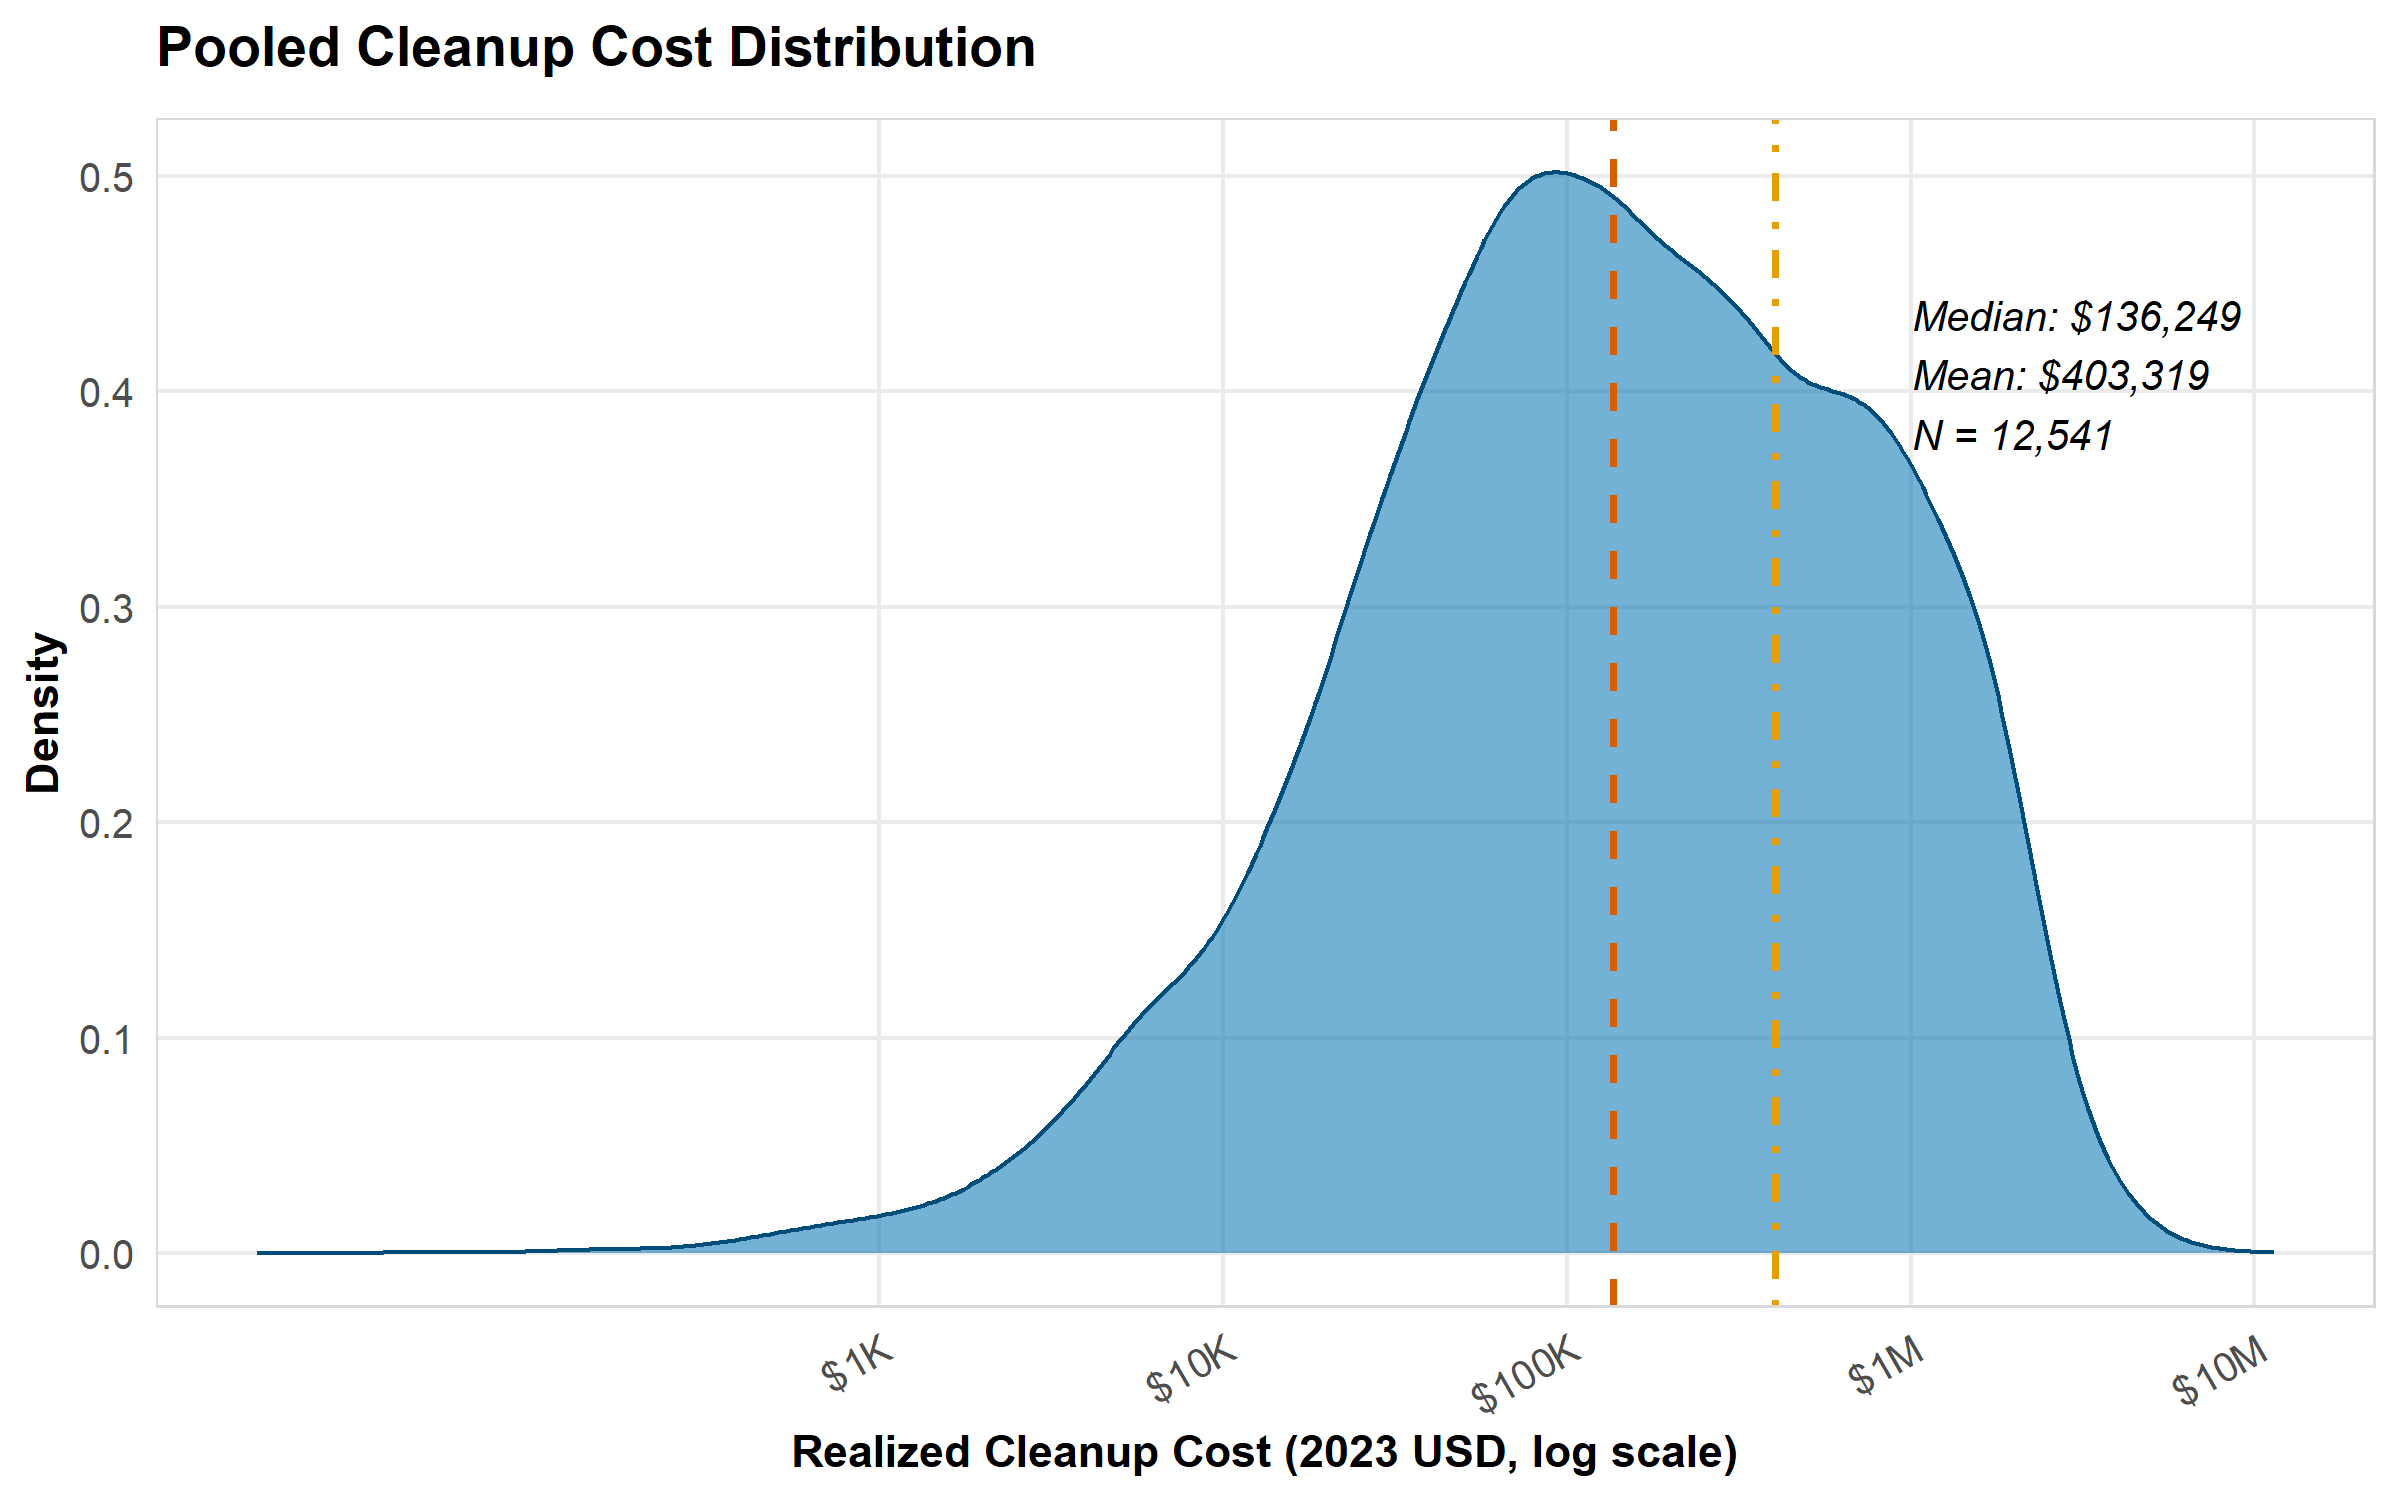
\includegraphics[height=0.72\textheight,keepaspectratio]{../../Output/Figures/Figure_cost_distribution_pooled.png}
\end{center}

\vfill

\centering\small\textit{$\sim$\,550,000 confirmed releases since 1988. Median cleanup \$136k; mean \$403k. Right tail dominates expected loss.}

\begin{tikzpicture}[remember picture, overlay]
\node[anchor=south west, inner sep=0pt] at ([xshift=10pt, yshift=10pt]current page.south west) {%
  \navbutton[cost-dist-states][fill=BerkeleyBlue, font=\tiny, inner sep=2pt]{Claims by state $\rightarrow$}%
};
\node[anchor=south east, inner sep=0pt] at ([xshift=-10pt, yshift=10pt]current page.south east) {%
  \navbutton[slide-data][fill=BerkeleyBlue!60, font=\tiny, inner sep=2pt]{$\leftarrow$ Data}%
};
\end{tikzpicture}
\end{frame}

\begin{frame}{Cleanup cost distribution by state (6 trust-fund states)}
\phantomsection\label{cleanup-cost-distribution-by-state-6-trust-fund-states}
\BerkeleyLightMode

\hypertarget{cost-dist-states}{}

\vspace{0.2cm}
\begin{center}
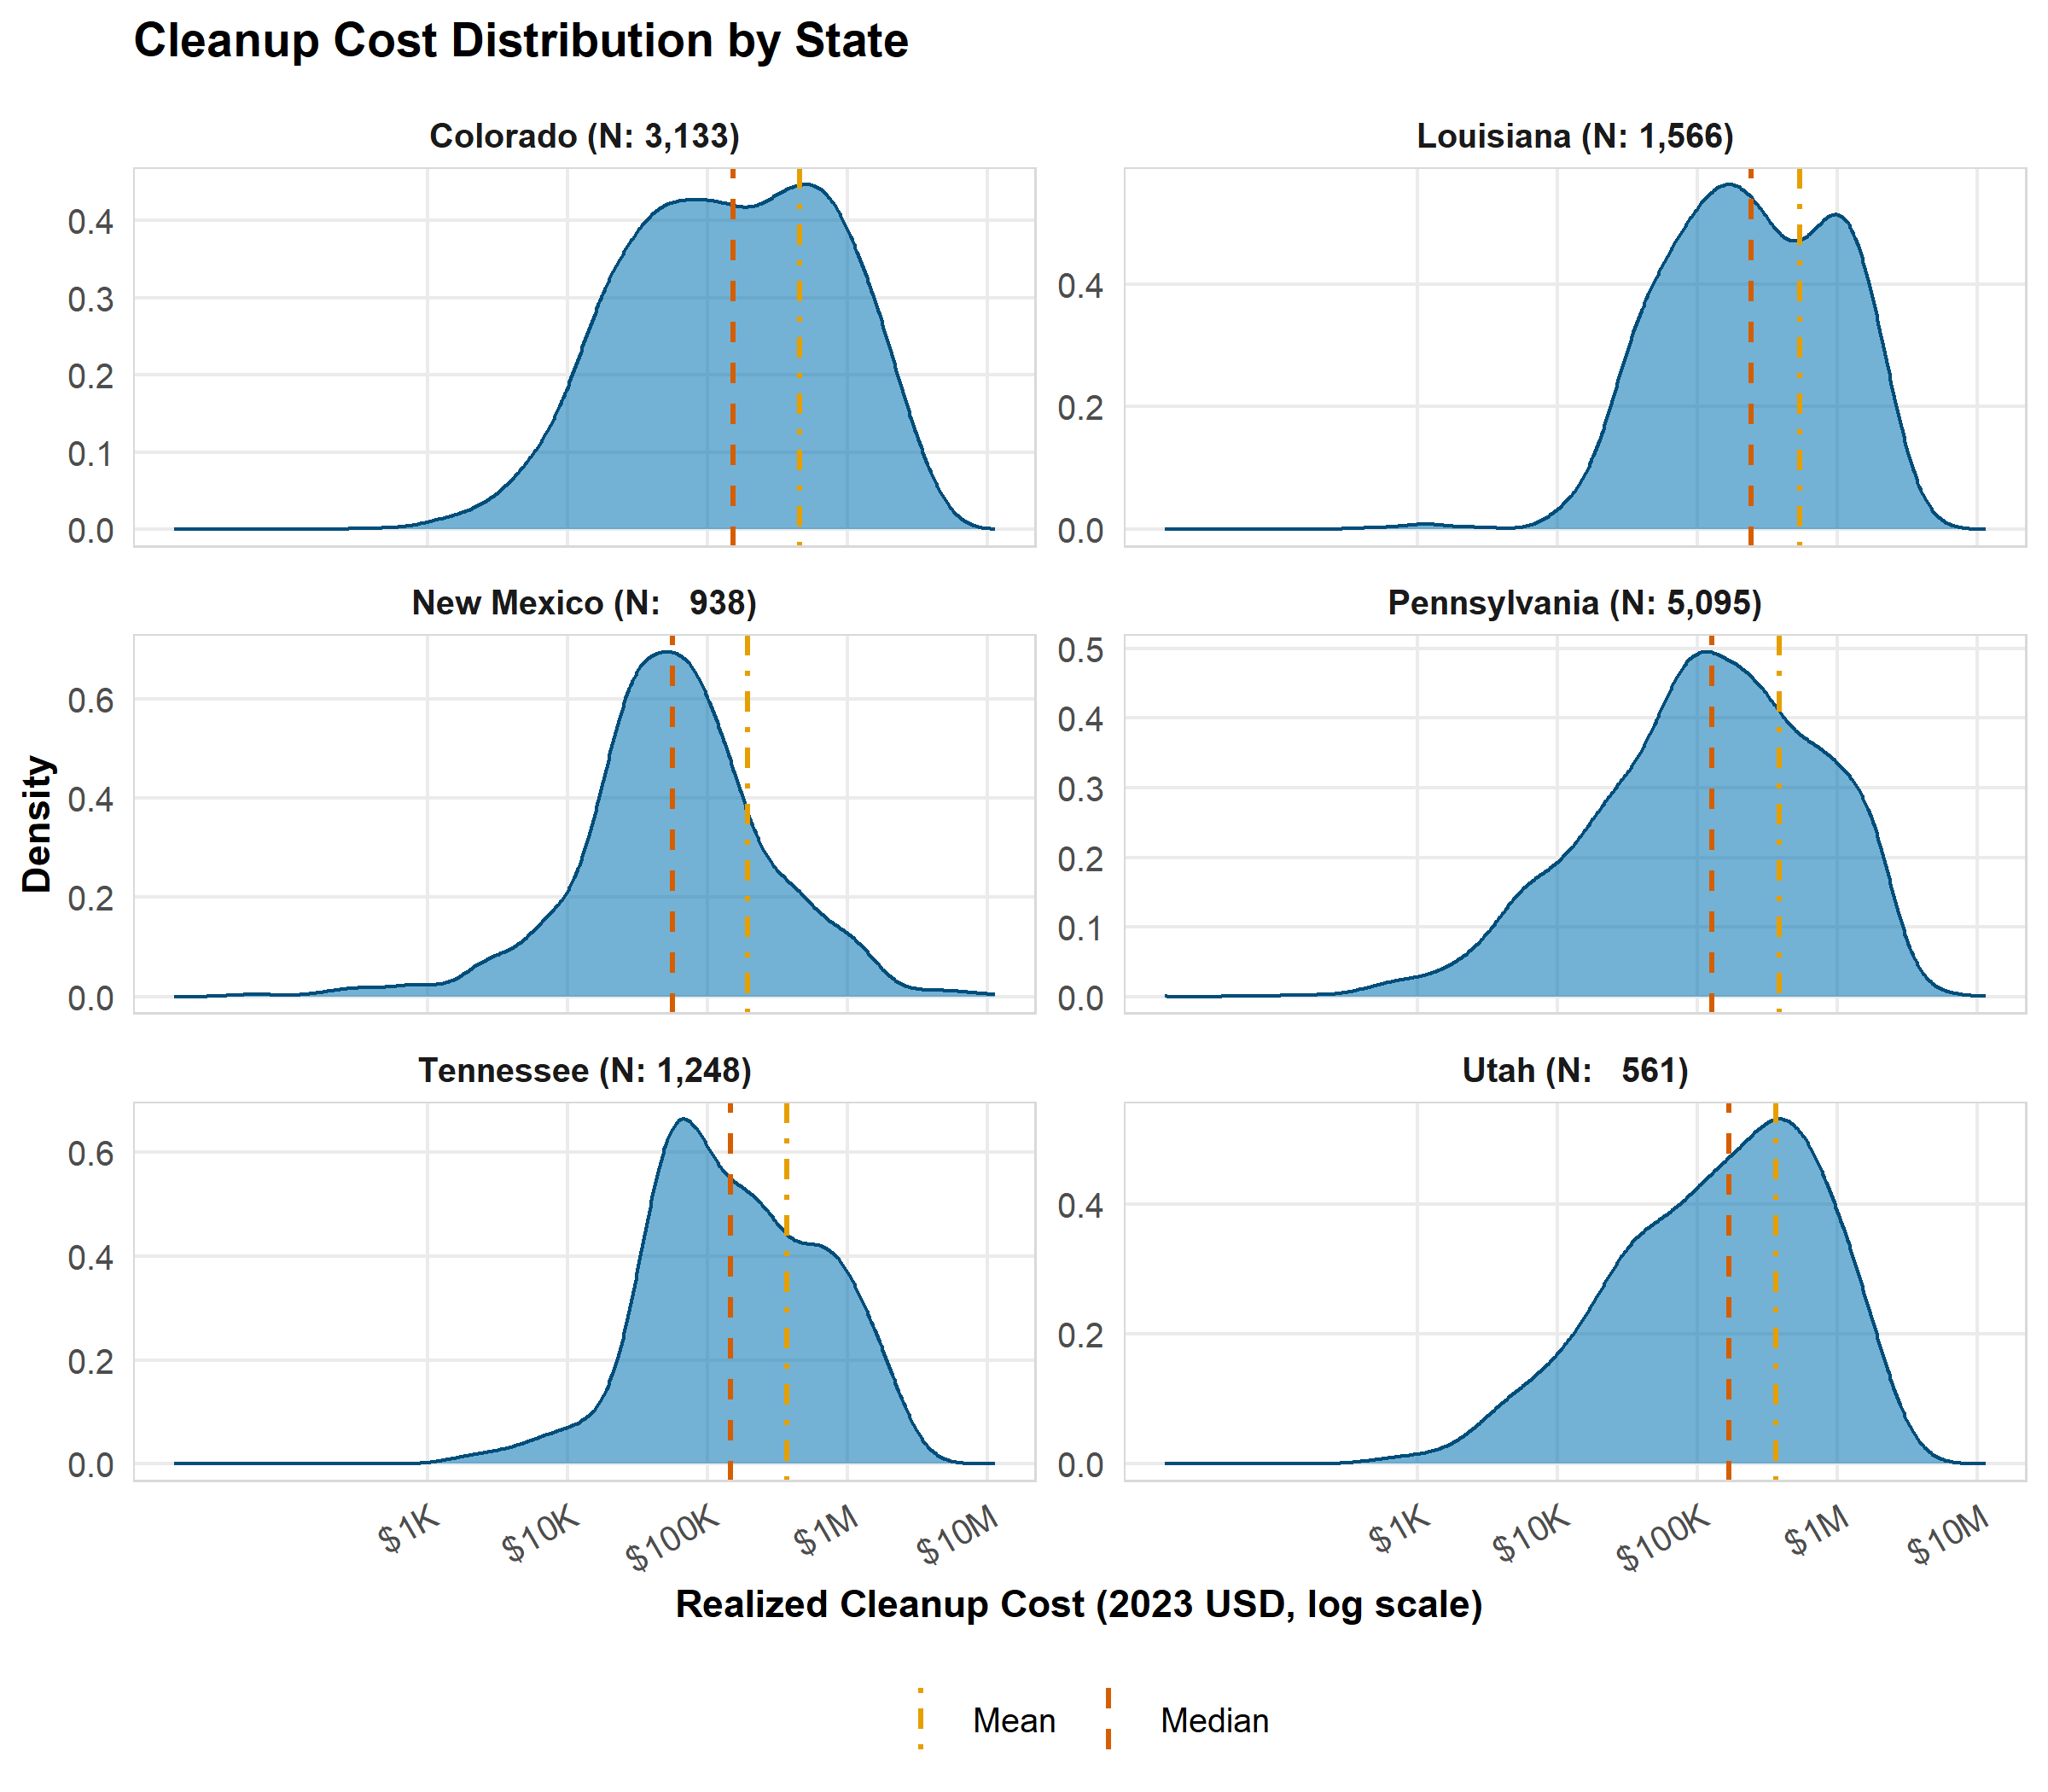
\includegraphics[width=0.92\textwidth,height=0.72\textheight,keepaspectratio]{../../Output/Figures/Figure_cost_distribution_by_state.png}
\end{center}

\vfill

\centering\small\textit{Per-site cleanup cost by state, deflated to 2023 dollars. State-level variation in the cost distribution; pooled distribution in prior slide masks meaningful right-tail heterogeneity.}

\begin{tikzpicture}[remember picture, overlay]
\node[anchor=south west, inner sep=0pt] at ([xshift=10pt, yshift=10pt]current page.south west) {%
  \navbutton[cost-dist-pooled][fill=BerkeleyBlue, font=\tiny, inner sep=2pt]{$\leftarrow$ Pooled distribution}%
};
\node[anchor=south east, inner sep=0pt] at ([xshift=-10pt, yshift=10pt]current page.south east) {%
  \navbutton[slide-data][fill=BerkeleyBlue!60, font=\tiny, inner sep=2pt]{$\leftarrow$ Data}%
};
\end{tikzpicture}
\end{frame}

\begin{frame}{Premium divergence: Texas vs.~control states (1992--2020)}
\phantomsection\label{premium-divergence-texas-vs.-control-states-19922020}
\BerkeleyLightMode

\hypertarget{premium-divergence}{}

\vspace{0.2cm}
\begin{center}
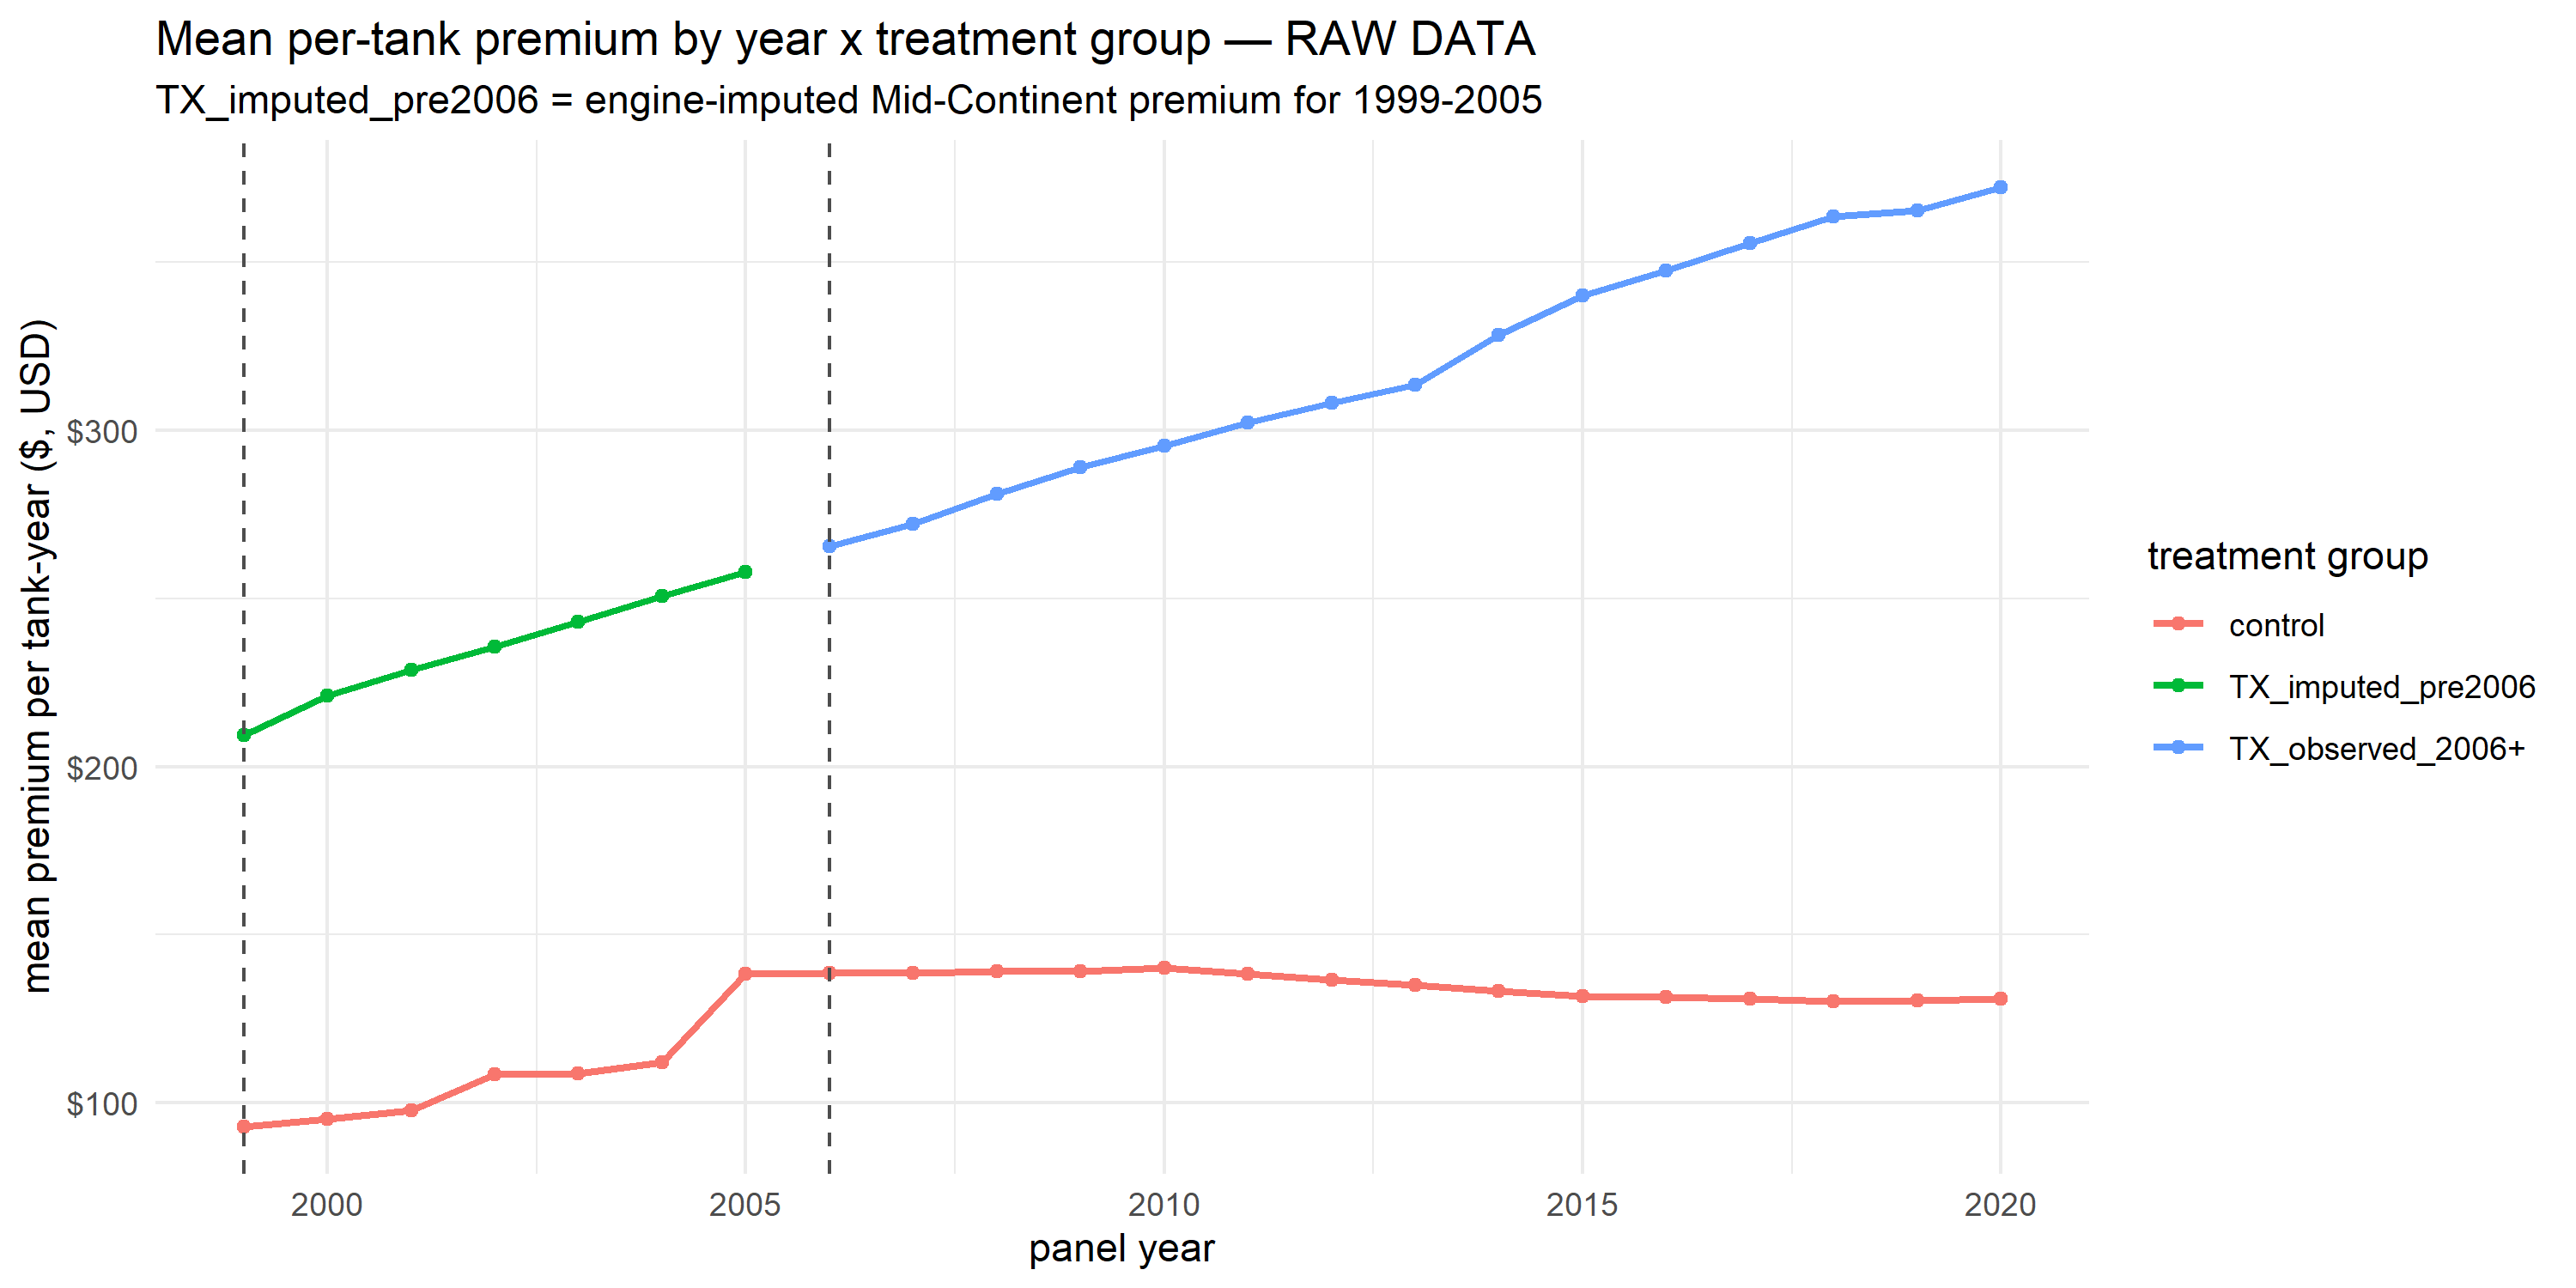
\includegraphics[width=0.92\textwidth,height=0.78\textheight,keepaspectratio]{../../Output/Figures/04e_Premium_by_Year_Treatment.png}
\end{center}

\vspace{0.1cm}

\centering\small\textit{Flat and parallel before 1998; sharp Texas divergence after the reform. Sets up the DiD without showing it.}

\begin{tikzpicture}[remember picture, overlay]
\node[anchor=south east, inner sep=0pt] at ([xshift=-10pt, yshift=10pt]current page.south east) {%
  \navbutton[slide-data][fill=BerkeleyBlue!60, font=\tiny, inner sep=2pt]{$\leftarrow$ Data}%
};
\end{tikzpicture}
\end{frame}

\begin{frame}{Risk is predictable: the age-hazard gradient (setup)}
\phantomsection\label{risk-is-predictable-the-age-hazard-gradient-setup}
\BerkeleyLightMode

\textbf{Estimand.} Annual first-release hazard in the never-yet-leaked
risk set:

\[
h(t \mid x) \;=\; P\bigl(\,\text{first confirmed release in year } t \mid \text{no prior release}, \; x\,\bigr)
\]

In plain words: given what an underwriter can observe at the start of a
policy year, what's the probability of a claim?

\textbf{Model.} Penalized logistic regression on the pre-treatment
panel:

\begin{itemize}
\tightlist
\item
  \(x\): 3-year age bins fully interacted with wall construction; state
  FE; fuel and portfolio controls
\item
  Lasso variable selection; inverse-frequency weights for the 0.70\%
  base rate
\item
  Out-of-sample CV (10 folds); post-hoc recalibration to the empirical
  event rate
\end{itemize}

\textbf{Sample.} 3.93M pre-treatment facility-years; \(27{,}455\)
confirmed first-release events.

\(\hat h(x)\) feeds the next figure and the structural-model hazard
\(h(a_t, W_i)\).
\end{frame}

\begin{frame}{Single-walled tanks drive the age-hazard gradient}
\phantomsection\label{single-walled-tanks-drive-the-age-hazard-gradient}
\BerkeleyLightMode

\vspace{0.2cm}
\begin{center}
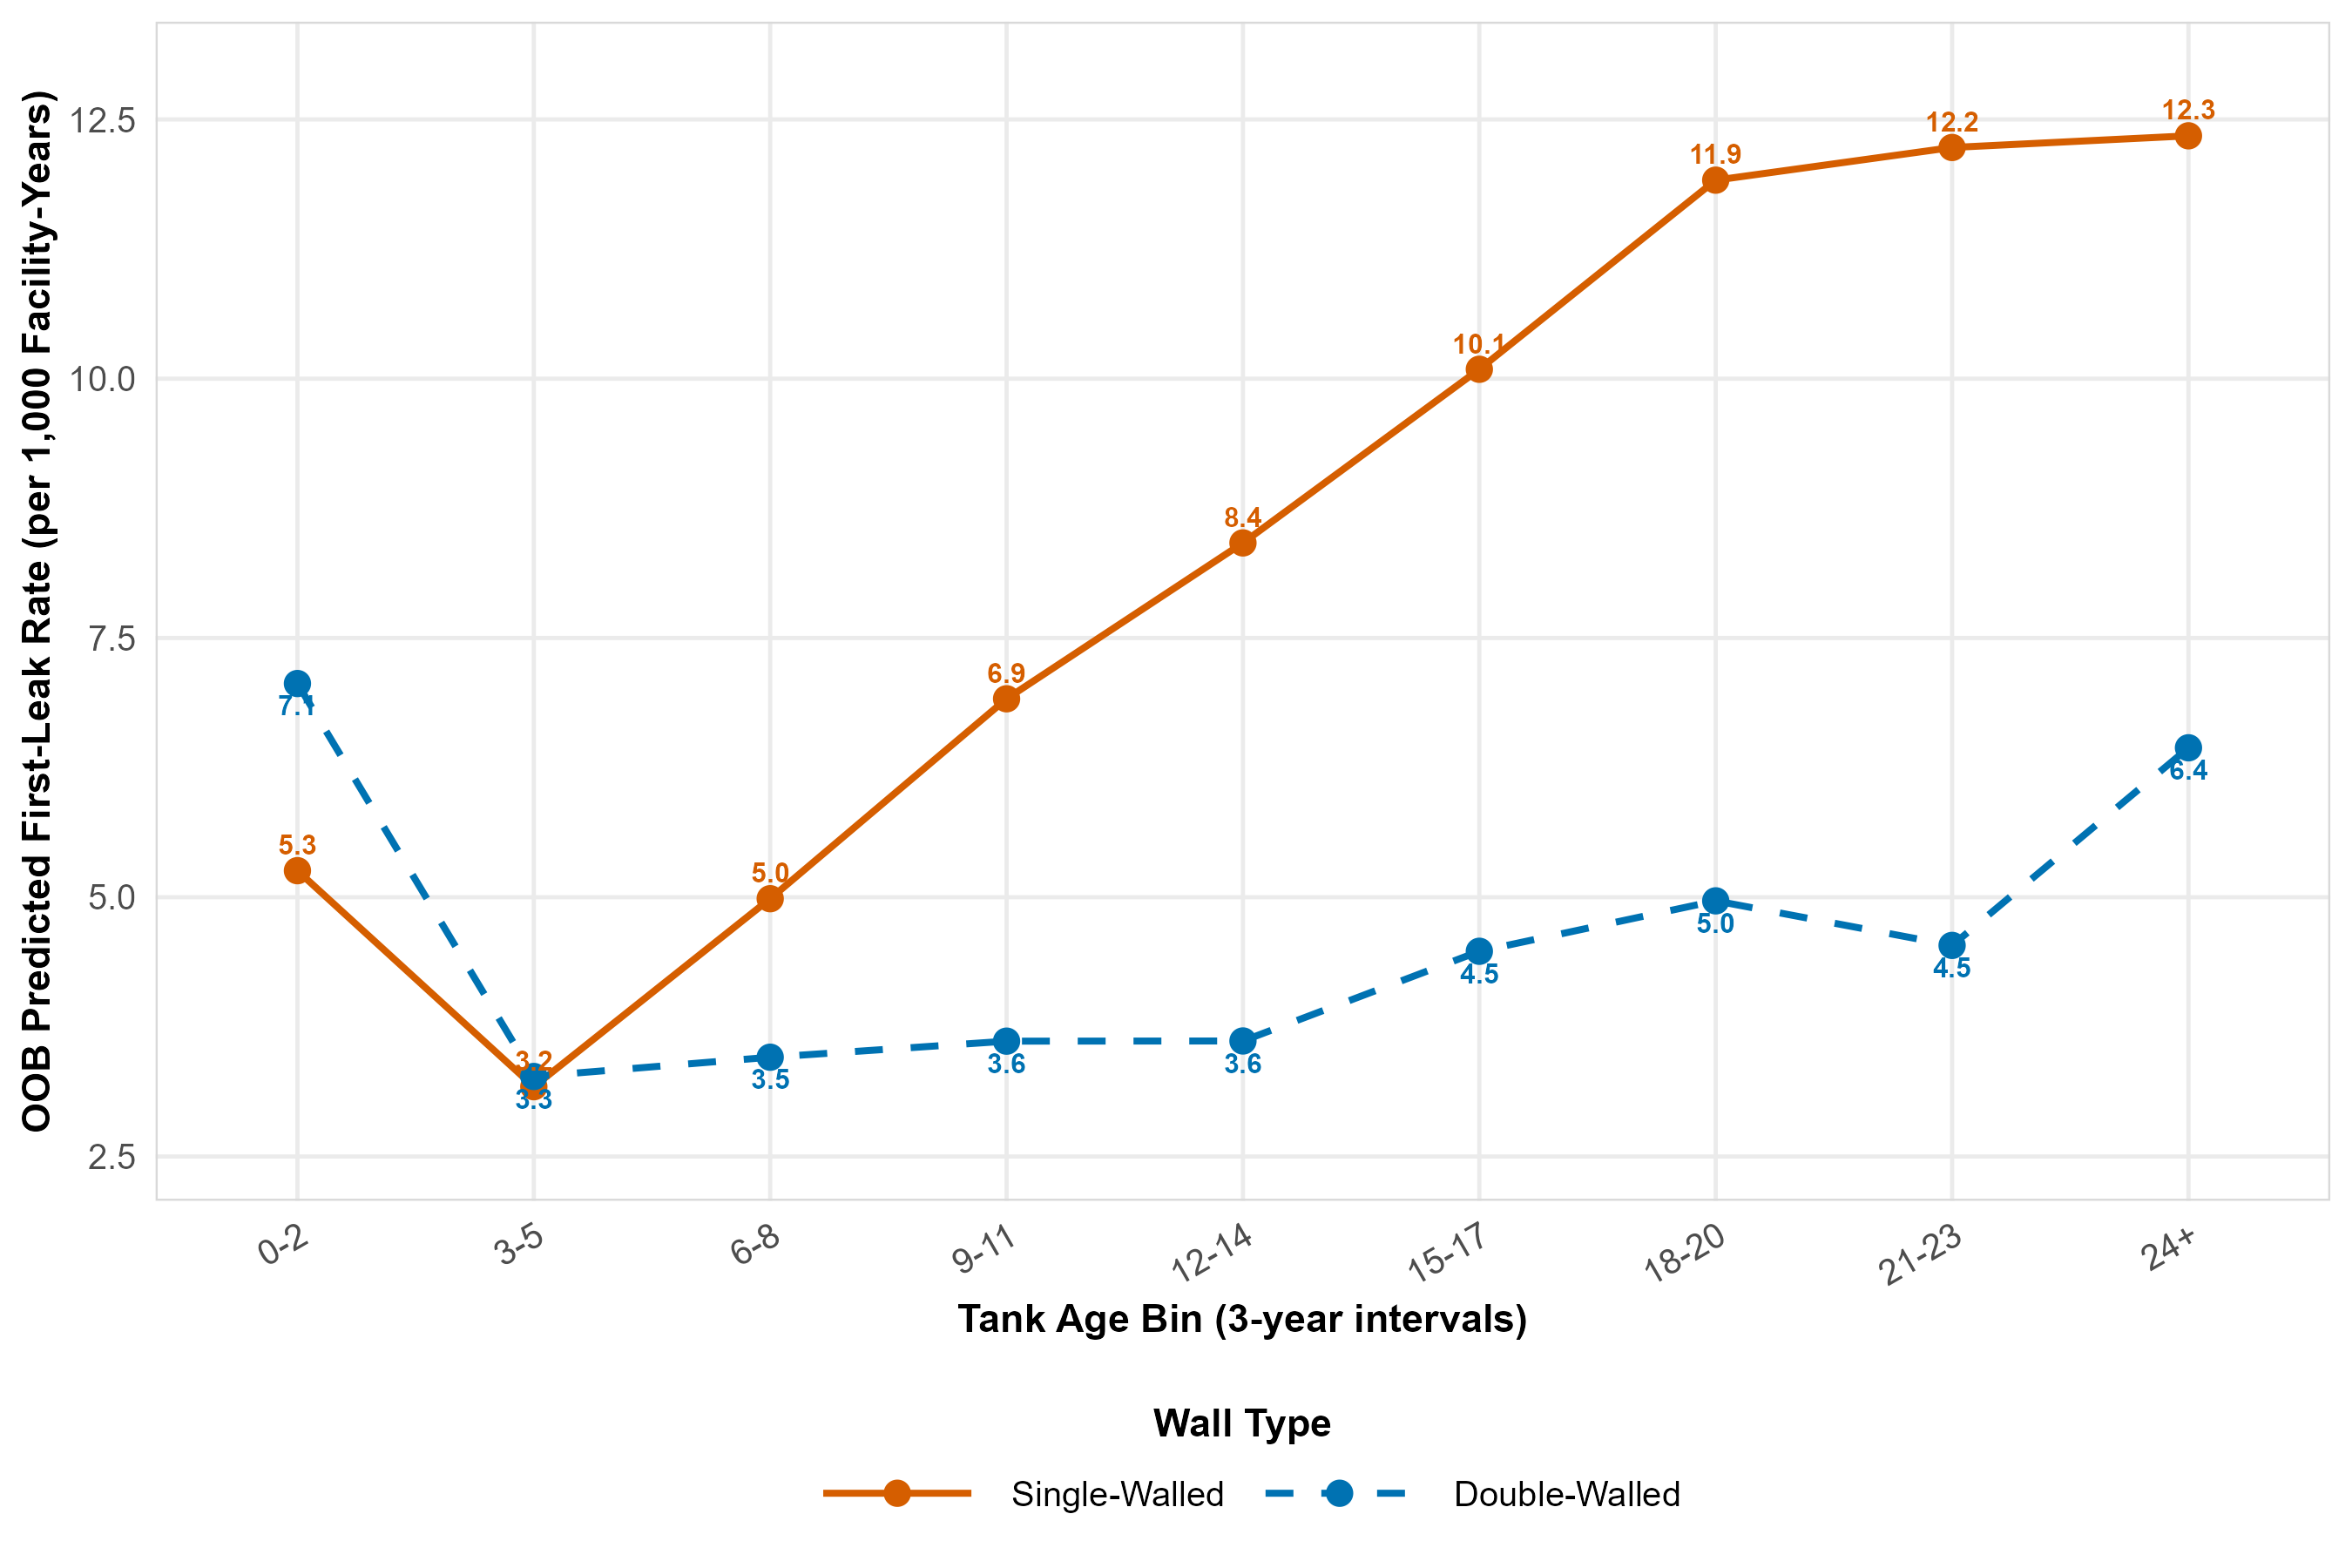
\includegraphics[width=0.92\textwidth,height=0.78\textheight,keepaspectratio]{../../Output/Figures/Figure_CV_CellRisk.png}
\end{center}

\begin{tikzpicture}[remember picture, overlay]
\node[anchor=south west, inner sep=0pt] at ([xshift=10pt, yshift=10pt]current page.south west) {%
  \navbutton[cell-gof][fill=BerkeleyBlue, font=\tiny, inner sep=2pt]{Goodness of fit $\rightarrow$}%
};
\end{tikzpicture}
\end{frame}

\begin{frame}{The insurance market: how Texas premiums are built}
\phantomsection\label{the-insurance-market-how-texas-premiums-are-built}
\BerkeleyLightMode

\textbf{Texas} --- rebuilt from major Texas UST insurer's rate filings
(SERFF, 2006--2024):

\[P_{ijt} \;=\; \text{Base}_t \;\times\; \text{ILF}_{it} \;\times\; \Bigl(1 \;+\; \sum_{k} \lambda_{k,t}\, X_{ijt,k}\Bigr)\]

\begin{itemize}
\tightlist
\item
  \(\text{Base}_t\): per-tank base rate, four filing periods
\item
  \(\text{ILF}_{it}\): increased-limit factor; fix coverage at
  federal-minimum \$1M/\$1M
\item
  \(X_{ijt}\): tank age, wall, piping, leak-detection technology
\item
  \(\lambda_{k,t}\): additive credits/debits from the filed schedule
\end{itemize}

\textbf{Control states} --- state financial-responsibility fund records:
a per-tank annual assessment, largely flat across years and tank
characteristics.
\end{frame}

\begin{frame}{Premiums track the risk we can predict}
\phantomsection\label{premiums-track-the-risk-we-can-predict}
\BerkeleyLightMode

\vspace{0.1cm}
\begin{center}
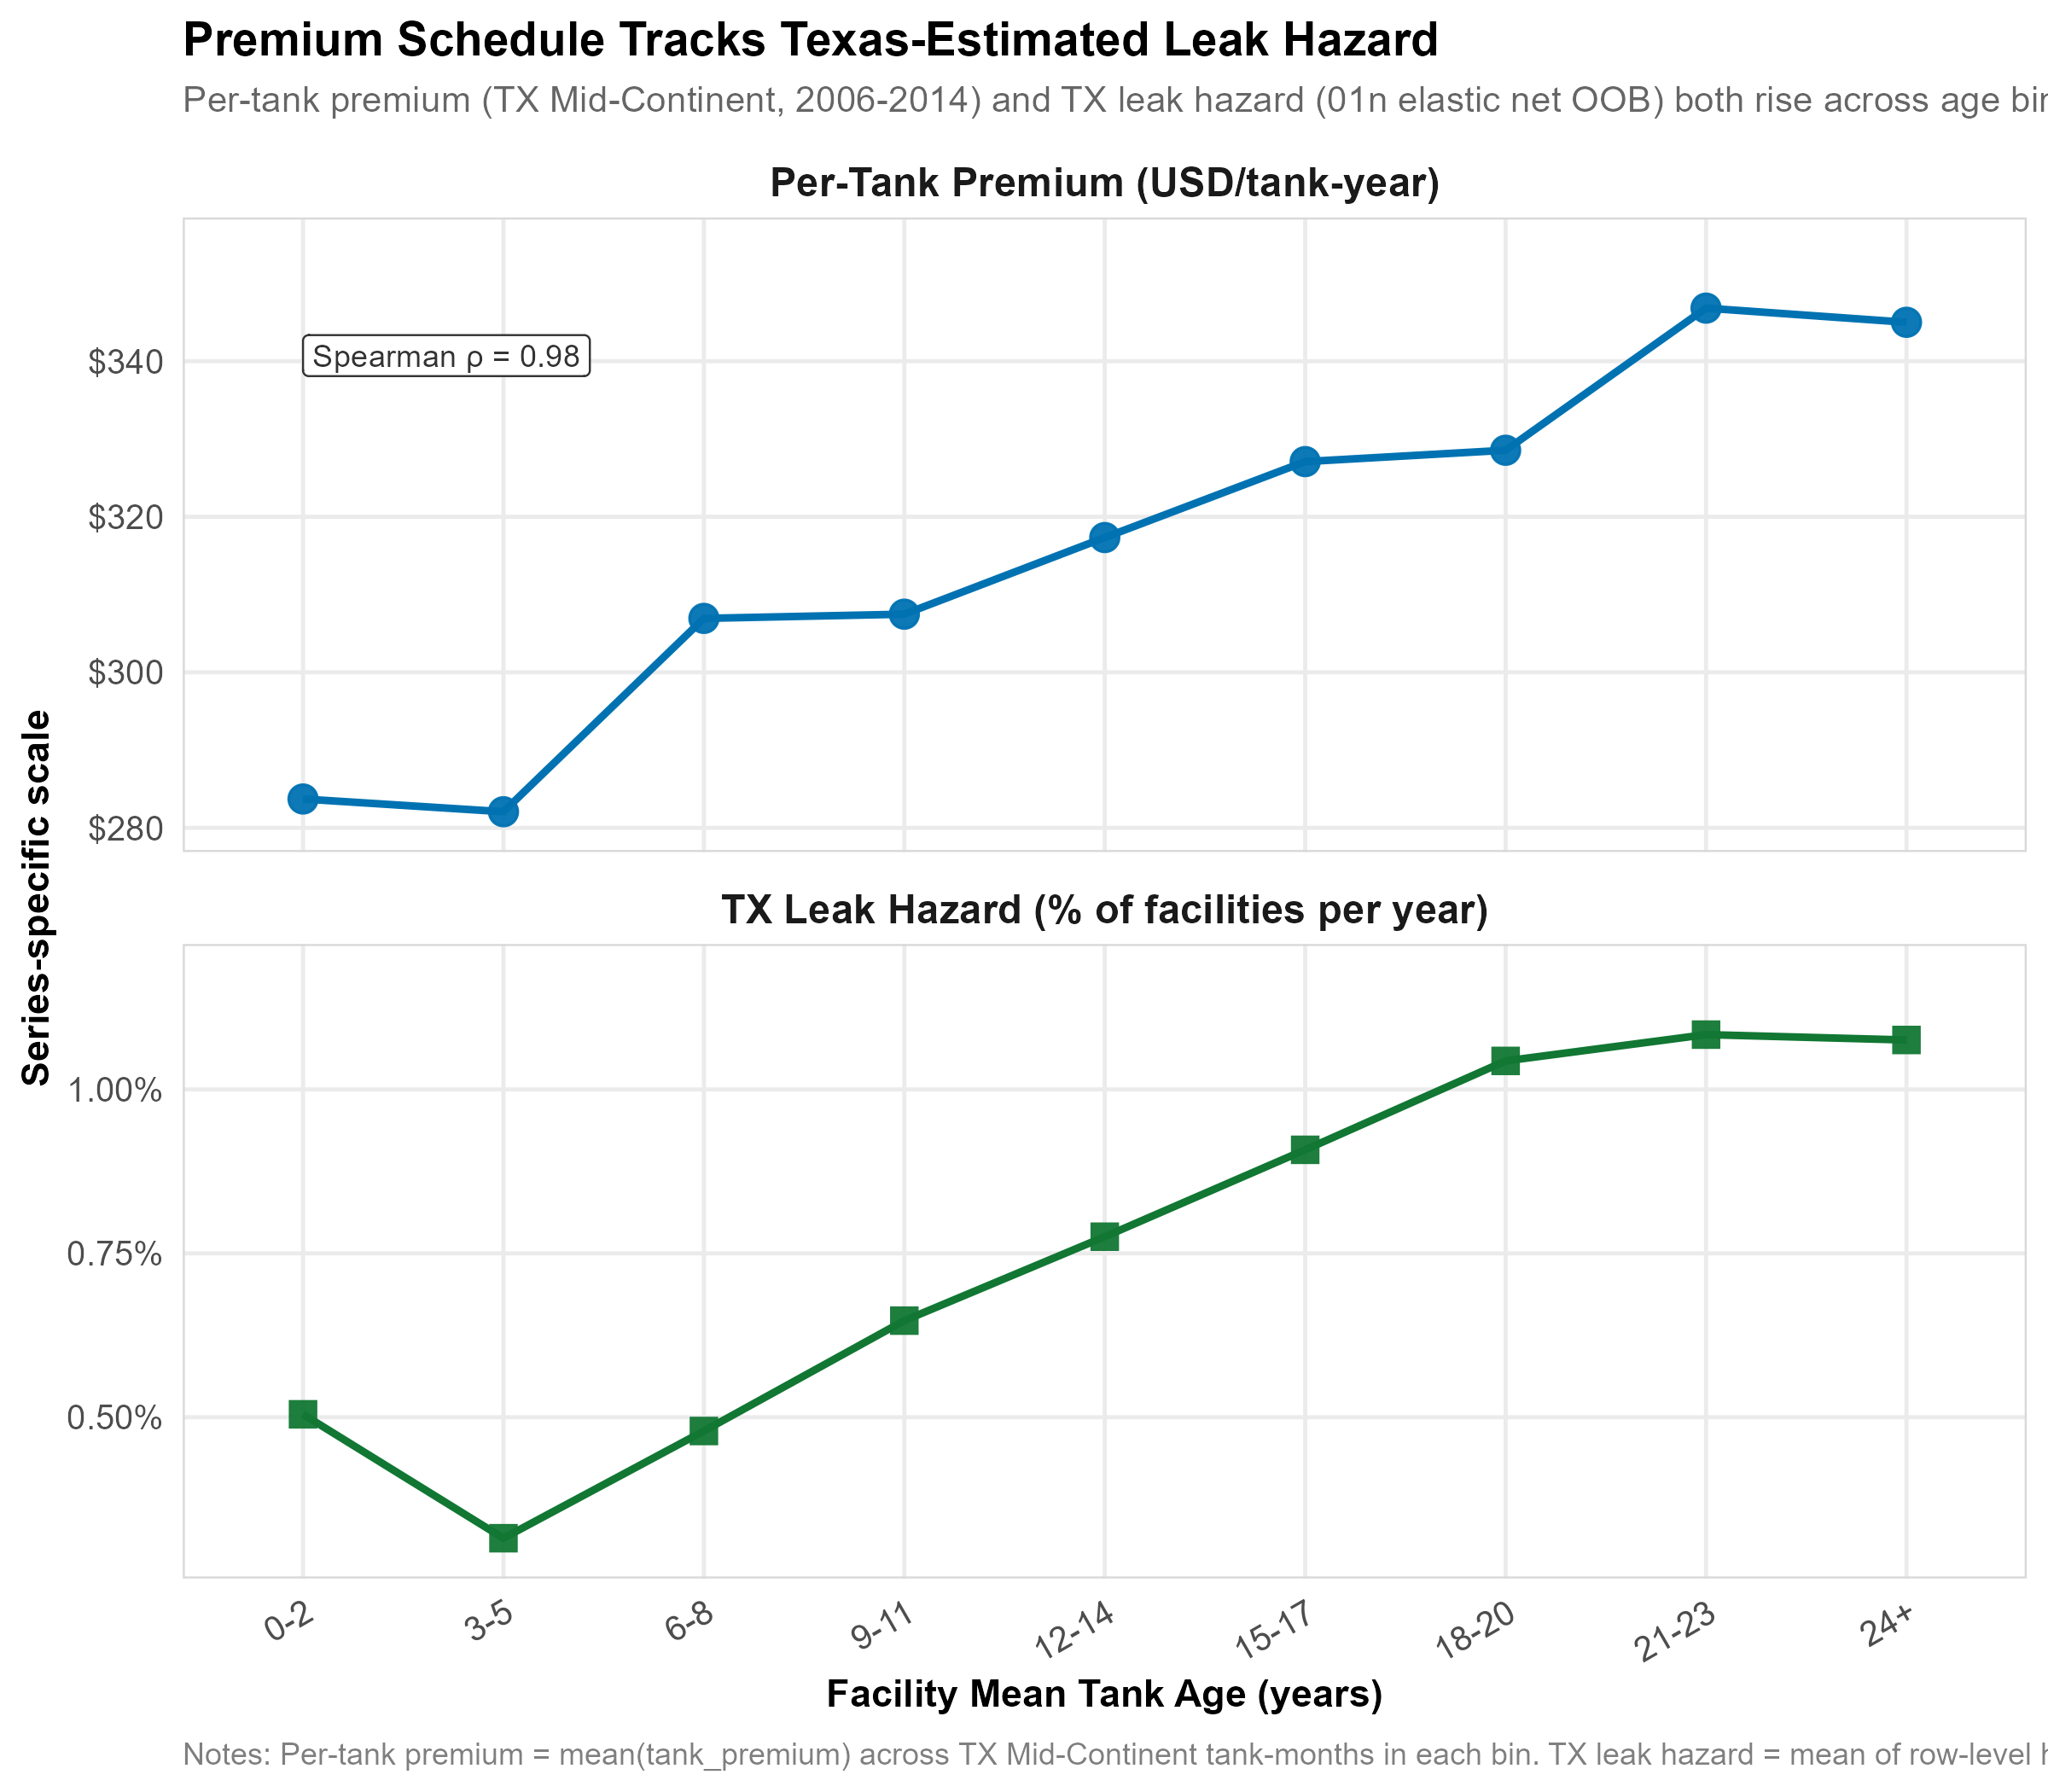
\includegraphics[height=0.80\textheight,keepaspectratio]{../../Output/Figures/Figure_Premium_vs_Hazard_Raw.png}
\end{center}

\begin{tikzpicture}[remember picture, overlay]
\node[anchor=south west, inner sep=0pt] at ([xshift=10pt, yshift=10pt]current page.south west) {%
  \navbutton[premium-vs-el][fill=BerkeleyBlue, font=\tiny, inner sep=2pt]{Predicted per-tank EL $\rightarrow$}%
};
\end{tikzpicture}
\end{frame}

\begin{frame}{}
\phantomsection\label{section-2}
\BerkeleyMode

\hypertarget{slide-rf}{}

\begin{center}
\Huge \textbf{Empirical Approach}
\end{center}

\begin{tikzpicture}[remember picture, overlay]
\node[anchor=south east, inner sep=0pt] at ([xshift=-10pt, yshift=10pt]current page.south east) {%
  \navbutton[slide-roadmap][fill=BerkeleyBlue!60, font=\tiny, inner sep=2pt]{$\leftarrow$ Roadmap}%
};
\end{tikzpicture}
\end{frame}

\begin{frame}{Research design: DiD with facility FE and cell-by-year FE}
\phantomsection\label{research-design-did-with-facility-fe-and-cell-by-year-fe}
\BerkeleyLightMode

\textbf{Static DiD.}

\[Y_{it} \;=\; \beta\,(\text{Texas}_{f(i)} \times \text{Post}_t) \;+\; \alpha_i \;+\; \delta_{ct} \;+\; \varepsilon_{it}\]

\textbf{Event study} (replaces single Post indicator with per-year
coefficients relative to 1998):

\[Y_{it} \;=\; \sum_{\tau \neq -1} \beta_\tau \cdot \bigl(\text{Texas}_{f(i)} \times \mathbf{1}[t - 1998 = \tau]\bigr) \;+\; \alpha_i \;+\; \delta_{ct} \;+\; \varepsilon_{it}\]

\begin{itemize}
\tightlist
\item
  \(\alpha_i\): facility FE. \(\delta_{ct}\): cell\(\times\)year FE with
  \(c = \{\text{wall}\times\text{fuel}\times\text{capacity}\times\text{install cohort}\}\)
\item
  \emph{Identifying variation:} within a single tank-vintage cell, in
  the same calendar year, \(\hat\beta\) is the change in the
  Texas-vs-control closure-rate gap before vs.~after Dec 22, 1998
\item
  \emph{Inference:} one treated unit \(\rightarrow\) Conley-Taber (2011)
  placebo inference; wild-cluster bootstrap at state level (18 clusters)
  as cross-check
\end{itemize}

\vspace{0.2cm}

\begin{tikzpicture}[remember picture, overlay]
\node[anchor=south east, inner sep=0pt] at ([xshift=-10pt, yshift=10pt]current page.south east) {%
  \navbutton[slide-roadmap][fill=BerkeleyBlue!60, font=\tiny, inner sep=2pt]{$\leftarrow$ Roadmap}%
};
\end{tikzpicture}
\end{frame}

\begin{frame}{}
\phantomsection\label{section-3}
\BerkeleyMode

\hypertarget{slide-results}{}

\begin{center}
\Huge \textbf{Results}
\end{center}

\begin{tikzpicture}[remember picture, overlay]
\node[anchor=south east, inner sep=0pt] at ([xshift=-10pt, yshift=10pt]current page.south east) {%
  \navbutton[slide-roadmap][fill=BerkeleyBlue!60, font=\tiny, inner sep=2pt]{$\leftarrow$ Roadmap}%
};
\end{tikzpicture}
\end{frame}

\begin{frame}{Event study: closure response in Texas}
\phantomsection\label{event-study-closure-response-in-texas}
\BerkeleyLightMode

\vspace{0.2cm}
\begin{center}
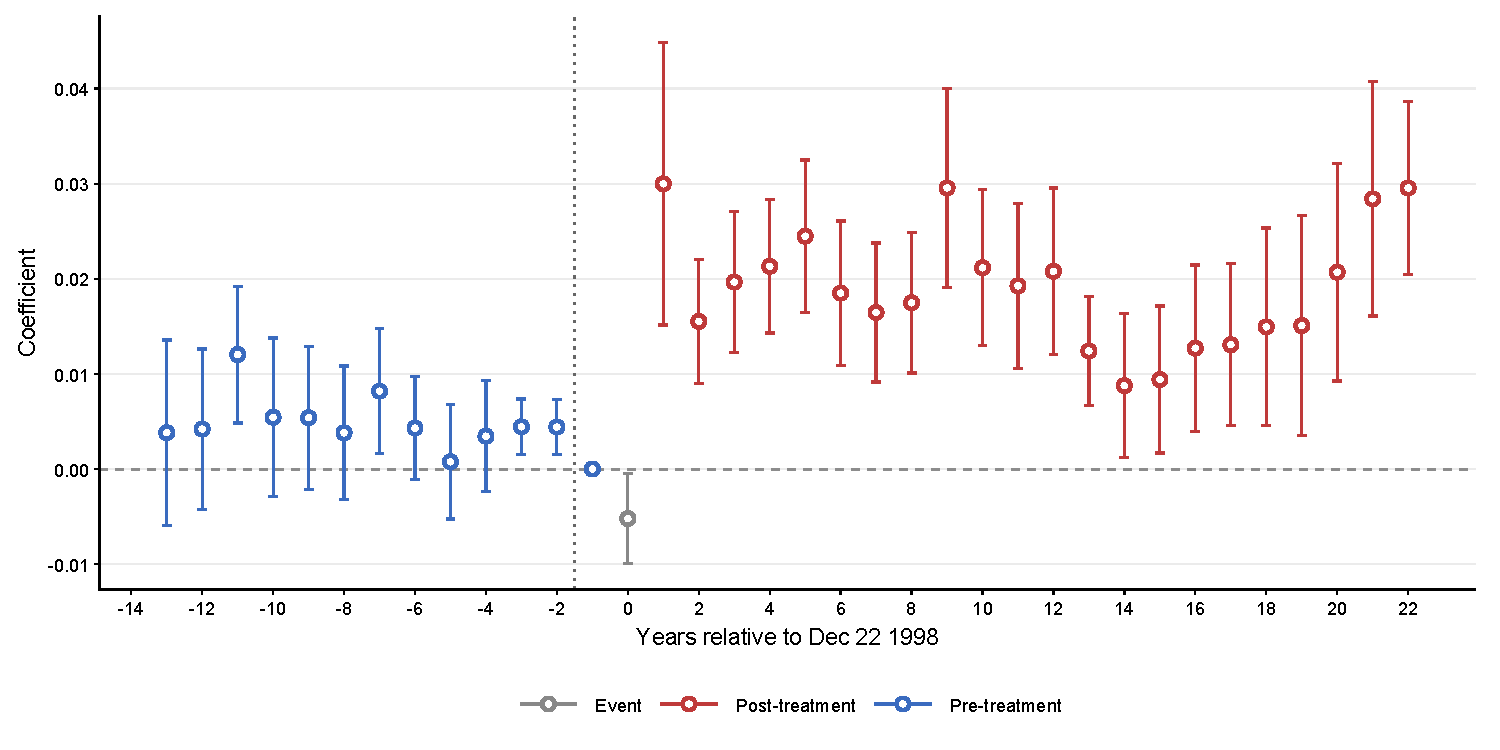
\includegraphics[width=0.92\textwidth,height=0.78\textheight,keepaspectratio]{../../Output/Figures/Fig_ES_Full.pdf}
\end{center}

\vspace{0.1cm}

\centering\small\textit{Pre-trends flat; sharp break at Dec 22, 1998; sustained post-treatment effect.}

\begin{tikzpicture}[remember picture, overlay]
\node[anchor=south east, inner sep=0pt] at ([xshift=-10pt, yshift=10pt]current page.south east) {%
  \navbutton[slide-roadmap][fill=BerkeleyBlue!60, font=\tiny, inner sep=2pt]{$\leftarrow$ Roadmap}%
};
\end{tikzpicture}
\end{frame}

\begin{frame}{ATT on Tank Closure: \(+1.58\) pp on a \(2.0\%\) Baseline}
\phantomsection\label{att-on-tank-closure-1.58-pp-on-a-2.0-baseline}
\BerkeleyLightMode

\vspace{0.15cm}
\begin{center}
\begingroup
\scriptsize
\setlength{\tabcolsep}{5pt}
\renewcommand{\arraystretch}{0.95}

\begingroup
\centering
\begin{tabular}{lcccc}
   \toprule
                                            & (1) Raw        & (2) + Fac FE         & (3) + Controls & (4) + Cell FE \\   
                                            & (1)            & (2)                  & (3)            & (4)\\  
   \midrule 
   Constant                                 & 0.0203$^{***}$ &                      &                &   \\   
                                            & (0.0022)       &                      &                &   \\   
   did\_term                                & 0.0106$^{***}$ & 0.0338$^{***}$       & 0.0350$^{***}$ & 0.0158$^{***}$\\   
                                            & (0.0022)       & ($1\times 10^{-6}$)  & (0.0015)       & (0.0040)\\   
   mandate\_release\_det                    &                &                      & -0.0039        &   \\   
                                            &                &                      & (0.0035)       &   \\   
   mandate\_spill\_overfill                 &                &                      & 0.0048$^{*}$   &   \\   
                                            &                &                      & (0.0025)       &   \\   
   mandate\_integrity                       &                &                      & 0.0085$^{***}$ &   \\   
                                            &                &                      & (0.0026)       &   \\   
    \\
   Observations                             & 9,761,982      & 9,761,982            & 9,761,982      & 9,761,044\\  
   R$^2$                                    & 0.00047        & 0.03550              & 0.03584        & 0.07745\\  
   Within R$^2$                             &                & 0.00218              & 0.00253        & 0.00036\\  
    \\
   panel\_id fixed effects                  &                & $\checkmark$         & $\checkmark$   & $\checkmark$\\   
   cell\_vintage\_year\_fe fixed effects    &                &                      &                & $\checkmark$\\   
   \bottomrule
\end{tabular}
\par\endgroup



\endgroup
\end{center}

\vfill

\centering

\textit{Cols add facility FE, then cell$\times$year FE. Col (3) is the headline.}

\begin{tikzpicture}[remember picture, overlay]
\node[anchor=south east, inner sep=0pt] at ([xshift=-10pt, yshift=10pt]current page.south east) {%
  \navbutton[slide-roadmap][fill=BerkeleyBlue!60, font=\tiny, inner sep=2pt]{$\leftarrow$ Roadmap}%
};
\end{tikzpicture}
\end{frame}

\begin{frame}{Heterogeneity: Pre-89 Vintage Drives the Effect}
\phantomsection\label{heterogeneity-pre-89-vintage-drives-the-effect}
\BerkeleyLightMode

\vspace{-0.1cm}
\begin{center}
\begingroup
\scriptsize
\setlength{\tabcolsep}{3pt}
\renewcommand{\arraystretch}{0.7}

\begingroup
\centering
\begin{tabular}{lcccc}
   \toprule
                                            & (1) Raw        & (2) + Fac FE   & (3) + Controls & (4) + Cell FE \\   
                                            & (1)            & (2)            & (3)            & (4)\\  
   \midrule 
   Constant                                 & 0.0103$^{***}$ &                &                &   \\   
                                            & (0.0011)       &                &                &   \\   
   did\_term                                & 0.0048$^{***}$ & 0.0117$^{***}$ & 0.0114$^{***}$ & -0.0067$^{**}$\\   
                                            & (0.0011)       & (0.0028)       & (0.0029)       & (0.0031)\\   
   pre89\_cohort                            & 0.0135$^{***}$ & 0.0671$^{***}$ & 0.0696$^{***}$ &   \\   
                                            & (0.0023)       & (0.0062)       & (0.0060)       &   \\   
   did\_term $\times$ pre89\_cohort         & 0.0094$^{***}$ & 0.0382$^{***}$ & 0.0360$^{***}$ & 0.0309$^{***}$\\   
                                            & (0.0023)       & (0.0029)       & (0.0029)       & (0.0065)\\   
   mandate\_release\_det                    &                &                & -0.0114$^{**}$ &   \\   
                                            &                &                & (0.0040)       &   \\   
   mandate\_spill\_overfill                 &                &                & 0.0009         &   \\   
                                            &                &                & (0.0028)       &   \\   
   mandate\_integrity                       &                &                & 0.0044         &   \\   
                                            &                &                & (0.0030)       &   \\   
    \\
   Observations                             & 9,761,982      & 9,761,982      & 9,761,982      & 9,761,044\\  
   R$^2$                                    & 0.00249        & 0.04685        & 0.04750        & 0.07772\\  
   Within R$^2$                             &                & 0.01392        & 0.01460        & 0.00065\\  
    \\
   panel\_id fixed effects                  &                & $\checkmark$   & $\checkmark$   & $\checkmark$\\   
   cell\_vintage\_year\_fe fixed effects    &                &                &                & $\checkmark$\\   
   \bottomrule
\end{tabular}
\par\endgroup



\endgroup
\end{center}

\centering\scriptsize

\textit{Pre-89 ATT $= \hat\beta_0 + \hat\beta_1 \approx +3.1$ pp; post-88 ATT $= \hat\beta_0 \approx +0.6$ pp. A coincident Texas-wide shock predicts uniform response across vintage; only the insurance premium gradient predicts the 5$\times$ differential.}

\begin{tikzpicture}[remember picture, overlay]
\node[anchor=south west, inner sep=0pt] at ([xshift=10pt, yshift=10pt]current page.south west) {%
  \navbutton[vintage-forest][fill=BerkeleyBlue, font=\tiny, inner sep=2pt]{ATT by install year $\rightarrow$}%
};
\node[anchor=south east, inner sep=0pt] at ([xshift=-10pt, yshift=10pt]current page.south east) {%
  \navbutton[slide-roadmap][fill=BerkeleyBlue!60, font=\tiny, inner sep=2pt]{$\leftarrow$ Roadmap}%
};
\end{tikzpicture}
\end{frame}

\begin{frame}{LUST discovery falls under risk-based pricing}
\phantomsection\label{lust-discovery-falls-under-risk-based-pricing}
\BerkeleyLightMode

\vspace{0.2cm}
\begin{center}
\begingroup
\footnotesize
\renewcommand{\arraystretch}{1.05}
\begin{tabular}{lcc}
\toprule
Outcome & Pre-reform ctrl mean & TX $\times$ Post \\
\midrule
Any leak found this year                       & 1.73\% & $-$1.27\,pp\textsuperscript{***} \\
                                               &        & (0.0032)                         \\
\midrule
\multicolumn{3}{l}{\textit{By how the leak was discovered:}}                                \\
\hspace{0.5em}Routine monitoring               & 1.16\% & $-$0.76\,pp\textsuperscript{***} \\
\hspace{0.5em}\textit{(no closure in $\pm$60d)}&        & (0.0021)                         \\
\hspace{0.5em}Closure-inspection finding       & 0.61\% & $-$0.51\,pp\textsuperscript{**}  \\
\hspace{0.5em}\textit{(closure within 60d)}    &        & (0.0017)                         \\
\midrule
$N$ facility-years & \multicolumn{2}{c}{4{,}650{,}240}                                                  \\
Sample             & \multicolumn{2}{c}{Incumbent (alive at Dec 22, 1998)}                             \\
FE                 & \multicolumn{2}{c}{Facility + cell $\times$ year; cluster by state}    \\
\bottomrule
\end{tabular}

\endgroup
\end{center}

\vspace{0.1cm}

\centering\small\textit{Leak discovery falls $1.27$ pp on a $1.73\%$ base; both routine-monitoring and closure-inspection findings decline.}

\begin{tikzpicture}[remember picture, overlay]
\node[anchor=south east, inner sep=0pt] at ([xshift=-10pt, yshift=10pt]current page.south east) {%
  \navbutton[slide-roadmap][fill=BerkeleyBlue!60, font=\tiny, inner sep=2pt]{$\leftarrow$ Roadmap}%
};
\end{tikzpicture}
\end{frame}

\begin{frame}{Closure composition shifts toward replacement}
\phantomsection\label{closure-composition-shifts-toward-replacement}
\BerkeleyLightMode

\vspace{0.05cm}
\begin{center}
\begingroup
\let\small\scriptsize
\scriptsize
\renewcommand{\arraystretch}{0.85}
\small
\begin{tabular}{lcc}
\toprule
Outcome (conditional on closing) & Pre-reform ctrl mean & TX $\times$ Post \\
\midrule
Facility closes all tanks this year     & 70.9\%       & $+$6.5\,pp\textsuperscript{***} \\
                                        &              & (0.019)                          \\
Has a permanent closure (no replace)    & 88.3\%       & $-$6.2\,pp\textsuperscript{***} \\
                                        &              & (0.012)                          \\
Has a replacement closure (upgrade)     & 12.0\%       & $+$6.3\,pp\textsuperscript{***} \\
                                        &              & (0.013)                          \\
Any DW tank installed                   & 4.1\%        & $-$1.4\,pp\textsuperscript{*}   \\
                                        &              & (0.007)                          \\
Net tank change (count)                 & $-$1.905     & $+$0.020                         \\
                                        &              & (0.085)                          \\
Capacity change (gal)                   & $-$100{,}394 & $-$1{,}397                       \\
                                        &              & (5{,}715)                        \\
\midrule
$N$ closing facility-years & \multicolumn{2}{c}{59{,}107}                                                       \\
Sample                     & \multicolumn{2}{c}{Incumbent, any\_closure $=1$}                                   \\
FE                         & \multicolumn{2}{c}{Facility + make\_model\_fac $\times$ year; cluster by state}    \\
\bottomrule
\end{tabular}

\endgroup
\end{center}

\vspace{0.05cm}

\centering\scriptsize\textit{Among closing facilities, RBP raises the replacement (upgrade) share and lowers permanent closures --- the margin the structural model recovers.}

\begin{tikzpicture}[remember picture, overlay]
\node[anchor=south east, inner sep=0pt] at ([xshift=-10pt, yshift=10pt]current page.south east) {%
  \navbutton[slide-roadmap][fill=BerkeleyBlue!60, font=\tiny, inner sep=2pt]{$\leftarrow$ Roadmap}%
};
\end{tikzpicture}
\end{frame}

\begin{frame}{What the reduced form cannot tell us}
\phantomsection\label{what-the-reduced-form-cannot-tell-us}
\BerkeleyLightMode

\textbf{The DiD identifies an average treatment effect. Three questions it cannot answer:}

\vspace{0.2cm}

\begin{enumerate}

\item \textbf{How large are the welfare effects in dollar terms?} The DiD gives a closure-rate gap, not a present-value welfare number on which to compare policies.

\item \textbf{What would alternative policies (subsidy, Pigouvian surcharge, age mandate) actually do?} These were not implemented in Texas. Their welfare consequences are counterfactual.

\item \textbf{How far are we from first-best, and why?} Risk-based pricing is a partial fix: premiums price what the insurer can claim, but health damages are structurally unpriced. Quantifying the residual wedge needs the structural primitives.

\end{enumerate}

\vfill

\textbf{Recovering the structural parameters is the only way to answer these. The structural model is not an add-on, it is required.}

\begin{tikzpicture}[remember picture, overlay]
\node[anchor=south east, inner sep=0pt] at ([xshift=-10pt, yshift=10pt]current page.south east) {%
  \navbutton[slide-structural][fill=BerkeleyBlue, font=\tiny, inner sep=2pt]{Structural model $\rightarrow$}%
};
\end{tikzpicture}
\end{frame}

\begin{frame}{}
\phantomsection\label{section-4}
\BerkeleyMode

\hypertarget{slide-structural}{}

\begin{center}
\Huge \textbf{Structural Model \& Counterfactuals}
\end{center}

\begin{tikzpicture}[remember picture, overlay]
\node[anchor=south east, inner sep=0pt] at ([xshift=-10pt, yshift=10pt]current page.south east) {%
  \navbutton[slide-roadmap][fill=BerkeleyBlue!60, font=\tiny, inner sep=2pt]{$\leftarrow$ Roadmap}%
};
\end{tikzpicture}
\end{frame}

\begin{frame}{What a facility looks like in the model}
\phantomsection\label{what-a-facility-looks-like-in-the-model}
\BerkeleyLightMode

\begin{itemize}
\tightlist
\item
  A facility is a set of underground tanks. Two things about each tank
  drive its cost and its risk: how old it is, and whether it is single-
  or double-walled.
\item
  The model describes a facility by the mix of tanks it holds: how many
  fall into each age-and-wall group, how much fuel it can store, and
  which pricing regime it faces.
\item
  Each year the owner decides what to do with that set: keep it as is,
  close some tanks, add new ones, or shut down for good.
\end{itemize}

\vfill

\centering\small\textit{Tanks are retired and replaced one at a time, so the real choice is how many to close or add, not a single keep-or-quit decision.}

\begin{tikzpicture}[remember picture, overlay]
\node[anchor=south east, inner sep=0pt] at ([xshift=-10pt, yshift=10pt]current page.south east) {%
  \navbutton[slide-roadmap][fill=BerkeleyBlue!60, font=\tiny, inner sep=2pt]{$\leftarrow$ Roadmap}%
};
\end{tikzpicture}
\end{frame}

\begin{frame}{State: the portfolio. Action: how many tanks to close or
add}
\phantomsection\label{state-the-portfolio.-action-how-many-tanks-to-close-or-add}
\BerkeleyLightMode

\[s = (\,n,\; G,\; \rho\,)\]

\begin{itemize}
\tightlist
\item
  \(n\): counts of tanks across 16 categories: wall type (single or
  double) \(\times\) eight 5-year age bins
\item
  \(G\): facility capacity bin; \(\rho\): pricing regime, fixed for the
  facility's life
\item
  A large but tractable state space, about \textbf{298{,}000} states in
  all
\end{itemize}

\vspace{0.15cm}

\textbf{Action} \((k,m)\): close \(k\) tanks, install \(m\).
\quad \((0,0)\) maintain \(\;\cdot\;\) \((k,0)\) downsize \(\;\cdot\;\)
\((k,m\ge 1)\) replace \(\;\cdot\;\) \(X\) exit.

\begin{itemize}
\tightlist
\item
  \textbf{Which} tanks leave is a rule, not a choice: oldest
  single-walled first. New tanks are double-walled (law).
\end{itemize}

\begin{tikzpicture}[remember picture, overlay]
\node[anchor=south west, inner sep=0pt] at ([xshift=10pt, yshift=10pt]current page.south west) {%
  \navbutton[model-coding][fill=BerkeleyBlue, font=\tiny, inner sep=2pt]{How a facility-year is coded $\rightarrow$}%
};
\node[anchor=south east, inner sep=0pt] at ([xshift=-10pt, yshift=10pt]current page.south east) {%
  \navbutton[slide-roadmap][fill=BerkeleyBlue!60, font=\tiny, inner sep=2pt]{$\leftarrow$ Roadmap}%
};
\end{tikzpicture}
\end{frame}

\begin{frame}{Each option's payoff: measured prices in, estimated
weights out}
\phantomsection\label{each-options-payoff-measured-prices-in-estimated-weights-out}
\BerkeleyLightMode

\begin{align*}
u_{(k,m)}(s) &= \varphi_G + \alpha_g - \estc{\gamma_p}\, P(n',\rho) - \estc{\gamma_r}\, OOP(n') - \estc{c^{\text{rem}}}\,k - \estc{c^{\text{inst}}}\,m &&\text{\small(operate)}\\[3pt]
u_X(s) &= \estc{\kappa_1}\, N(n) &&\text{\small(exit)}
\end{align*}

\vspace{0.1cm}

\begin{itemize}
\tightlist
\item
  \textbf{Measured first, not estimated:} the premium bill \(P\) (Texas
  filings or state fee), the leak hazard \(H\), out-of-pocket
  \(OOP = H \cdot D\), and the aging and capacity transitions
\item
  \textbf{Estimated} (in \estc{green}): \(\estc{\varphi_G}\) operating
  payoff by size, \(\estc{\gamma_p}\) premium weight,
  \(\estc{\gamma_r}\) out-of-pocket weight, \(\estc{c^{\text{rem}}}\)
  and \(\estc{c^{\text{inst}}}\) close / install costs,
  \(\estc{\kappa_1}\) exit value per tank
\item
  \(\estc{\gamma_p} = \estc{\gamma_r}\) is a testable restriction: does
  a premium dollar feel like an expected out-of-pocket dollar?
\end{itemize}

\begin{tikzpicture}[remember picture, overlay]
\node[anchor=south east, inner sep=0pt] at ([xshift=-10pt, yshift=10pt]current page.south east) {%
  \navbutton[slide-roadmap][fill=BerkeleyBlue!60, font=\tiny, inner sep=2pt]{$\leftarrow$ Roadmap}%
};
\end{tikzpicture}
\end{frame}

\begin{frame}{The dynamic choice: today's payoff vs.~operating next
year}
\phantomsection\label{the-dynamic-choice-todays-payoff-vs.-operating-next-year}
\BerkeleyLightMode

\[v_a(s) = u_a(s) + \beta\,\mathbb{E}\!\left[V(s') \mid s, a\right], \qquad V(s) = \log\!\Bigl(\, e^{v_{\text{maintain}}(s)} + e^{IV(s)} + e^{v_{\text{exit}}(s)} \,\Bigr)\]

\vspace{0.1cm}

\begin{itemize}
\tightlist
\item
  Each year the owner compares \textbf{maintain}, any \textbf{tank-work}
  option \((k,m)\), and \textbf{exit}, trading today's payoff against
  the value of operating next year
\item
  Nested logit: the tank-work options share a draw \(\lambda\) for the
  common decision to touch the tanks at all
\item
  \(\beta = 0.95\); estimated by nested pseudo-likelihood
  (Aguirregabiria \& Mira 2007). Eight economic parameters plus state
  fixed effects
\end{itemize}

\vfill

\centering\small\textit{Risk-based pricing makes the premium climb with age, so the value of holding old tanks falls and owners close or replace sooner.}

\begin{tikzpicture}[remember picture, overlay]
\node[anchor=south east, inner sep=0pt] at ([xshift=-10pt, yshift=10pt]current page.south east) {%
  \navbutton[slide-roadmap][fill=BerkeleyBlue!60, font=\tiny, inner sep=2pt]{$\leftarrow$ Roadmap}%
};
\end{tikzpicture}
\end{frame}

\begin{frame}{Why risk pricing is only a partial fix}
\phantomsection\label{why-risk-pricing-is-only-a-partial-fix}
\BerkeleyLightMode

\begin{itemize}
\tightlist
\item
  A leak costs society \(L + E\): cleanup \(L\) plus external health and
  water damage \(E\) beyond cleanup
\item
  The owner pays only the deductible \(D\) directly. The rest of
  cleanup, \(L - D\), falls on the insurer or fund. The external damage
  \(E\) is borne by no one in the market.
\end{itemize}

\vspace{0.15cm}
\begin{center}
\small
\renewcommand{\arraystretch}{1.3}
\begin{tabular}{lll}
\hline
\textbf{Regime} & \textbf{Owner internalizes} & \textbf{Wedge left open} \\
\hline
Uniform premium & roughly only the deductible $D$           & $(L - D) + E$ \\
Risk-based & $D$ plus part of $L - D$                  & $E$ plus the missing part of $L - D$ \\
First-best & the full $H\,(L + E)$ at the margin        & none \\
\hline
\end{tabular}
\end{center}

\vfill

\centering\small\textit{Social welfare $=$ producer surplus $-$ external damage $-$ government outlay. $E$ calibrated at \$50k per leak, with a band.}

\begin{tikzpicture}[remember picture, overlay]
\node[anchor=south east, inner sep=0pt] at ([xshift=-10pt, yshift=10pt]current page.south east) {%
  \navbutton[slide-roadmap][fill=BerkeleyBlue!60, font=\tiny, inner sep=2pt]{$\leftarrow$ Roadmap}%
};
\end{tikzpicture}
\end{frame}

\begin{frame}{Four counterfactuals (estimation in progress, no results
yet)}
\phantomsection\label{four-counterfactuals-estimation-in-progress-no-results-yet}
\BerkeleyLightMode

Once the portfolio model is estimated, we run four policy experiments:

\vspace{0.2cm}

\begin{enumerate}
\item \textbf{Uniform-premium Texas.} Texas keeps its state-run uniform premium. The welfare cost of the reform itself.
\item \textbf{First-best Pigouvian contract.} Exposure set to the full social cost $H(L+E)$. The welfare ceiling.
\item \textbf{Single-walled replacement subsidy.} Pay down the cost of replacing the riskiest tanks.
\item \textbf{Age mandate.} Force removal at age $A$.
\end{enumerate}

\vfill

\centering\small\textit{Each is judged by the margins it moves: closure, replacement, leaks, and welfare. No results yet; this is the plan for the summer.}

\begin{tikzpicture}[remember picture, overlay]
\node[anchor=south east, inner sep=0pt] at ([xshift=-10pt, yshift=10pt]current page.south east) {%
  \navbutton[slide-roadmap][fill=BerkeleyBlue!60, font=\tiny, inner sep=2pt]{$\leftarrow$ Roadmap}%
};
\end{tikzpicture}
\end{frame}

\begin{frame}{Appendix: Cell-Level Goodness of Fit}
\phantomsection\label{appendix-cell-level-goodness-of-fit}
\BerkeleyLightMode

\hypertarget{cell-gof}{}

\vspace{0.2cm}
\begin{center}
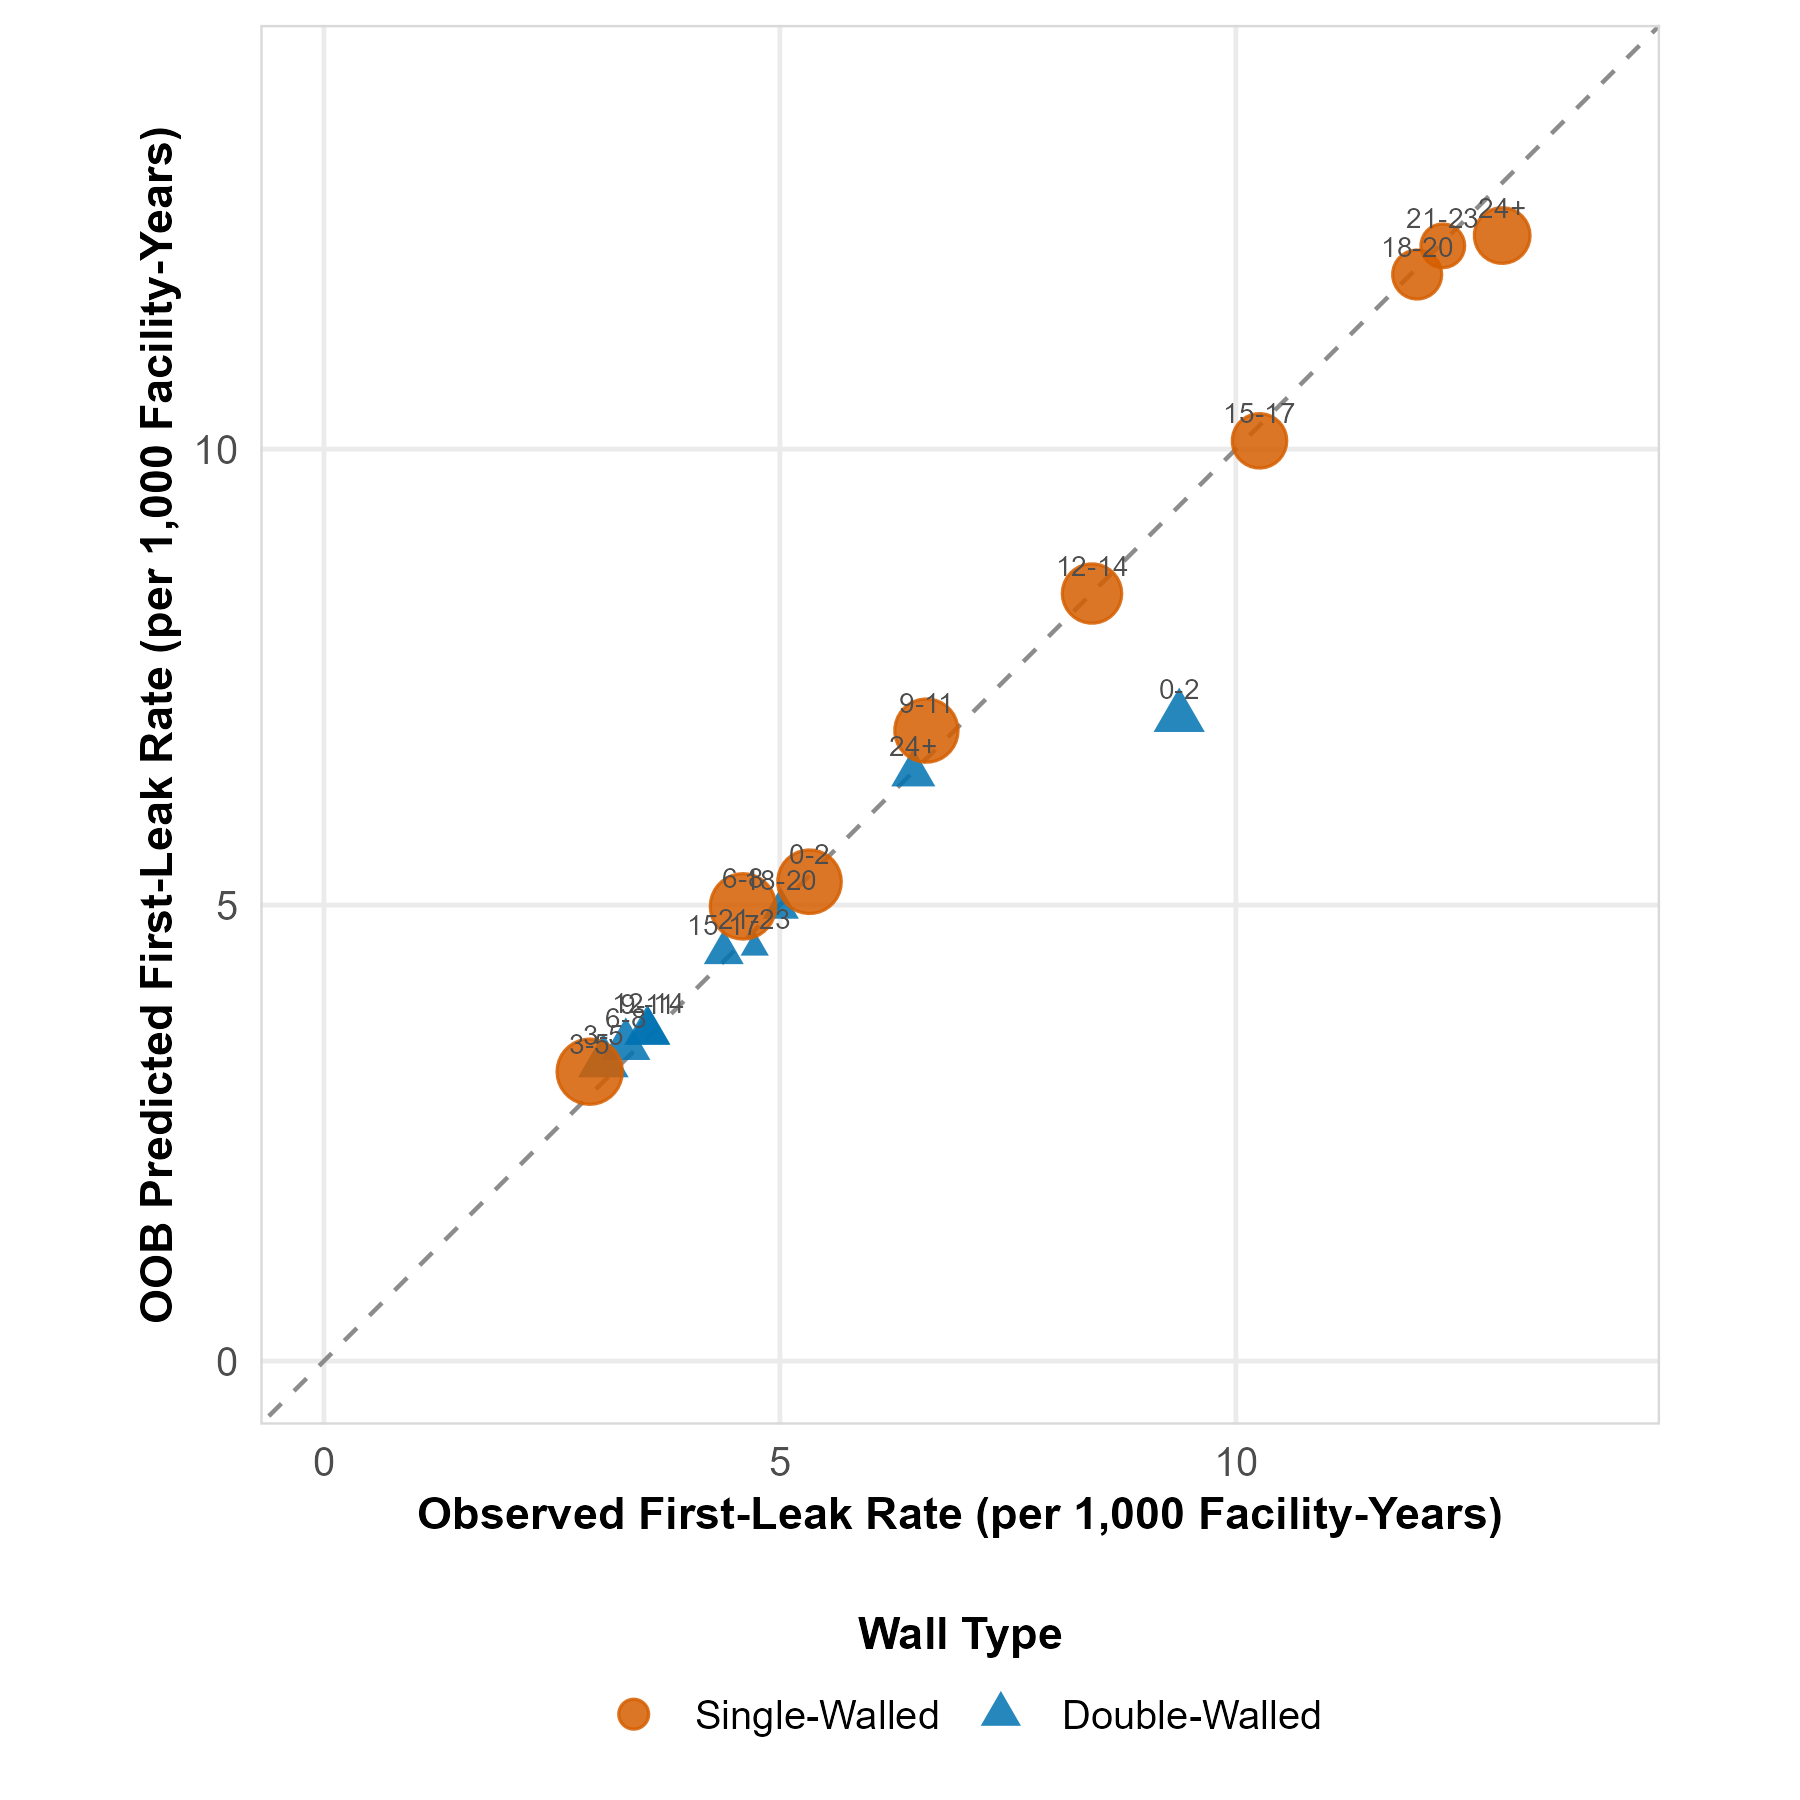
\includegraphics[width=0.92\textwidth,height=0.78\textheight,keepaspectratio]{../../Output/Figures/Figure_CV_CellRisk_GoF.png}
\end{center}

\begin{tikzpicture}[remember picture, overlay]
\node[anchor=south west, inner sep=0pt] at ([xshift=10pt, yshift=10pt]current page.south west) {%
  \navbutton[slide-data][fill=BerkeleyBlue, font=\tiny, inner sep=2pt]{$\leftarrow$ back}%
};
\end{tikzpicture}
\end{frame}

\begin{frame}{Appendix: ATT by installation vintage}
\phantomsection\label{appendix-att-by-installation-vintage}
\BerkeleyLightMode

\hypertarget{vintage-forest}{}

\vspace{0.2cm}
\begin{center}
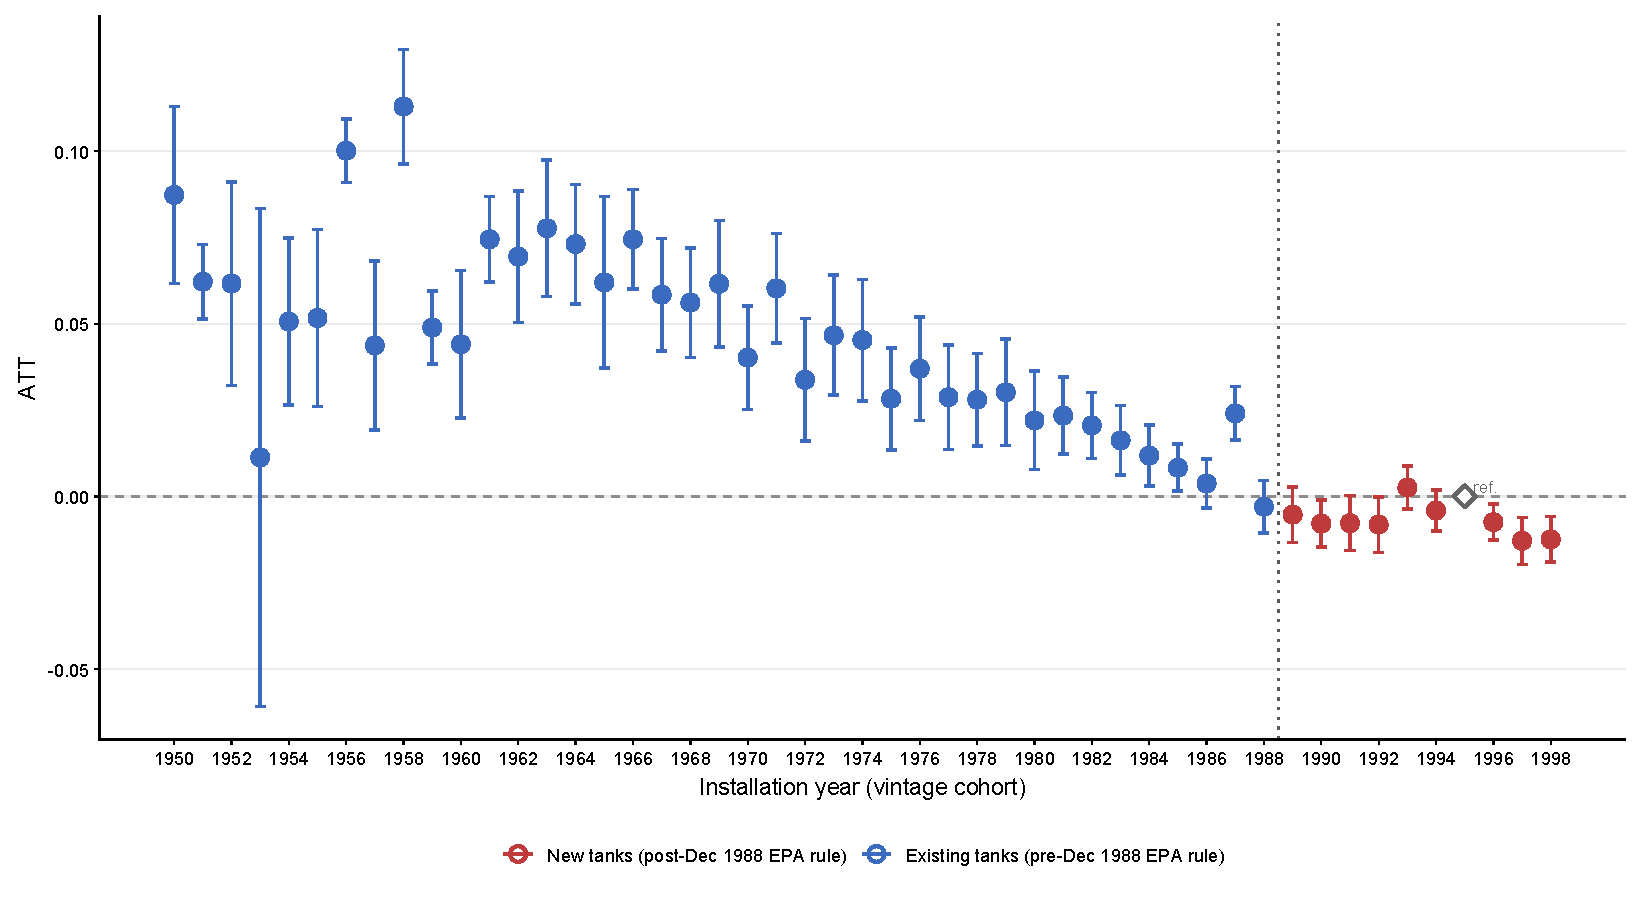
\includegraphics[width=0.92\textwidth,height=0.78\textheight,keepaspectratio]{../../Output/Figures/Fig_Vintage_Forest.pdf}
\end{center}

\begin{tikzpicture}[remember picture, overlay]
\node[anchor=south west, inner sep=0pt] at ([xshift=10pt, yshift=10pt]current page.south west) {%
  \navbutton[slide-results][fill=BerkeleyBlue, font=\tiny, inner sep=2pt]{$\leftarrow$ back}%
};
\end{tikzpicture}
\end{frame}

\begin{frame}{Appendix: Premium vs.~Per-Tank Expected Loss}
\phantomsection\label{appendix-premium-vs.-per-tank-expected-loss}
\BerkeleyLightMode

\hypertarget{premium-vs-el}{}

\vspace{0.2cm}
\begin{center}
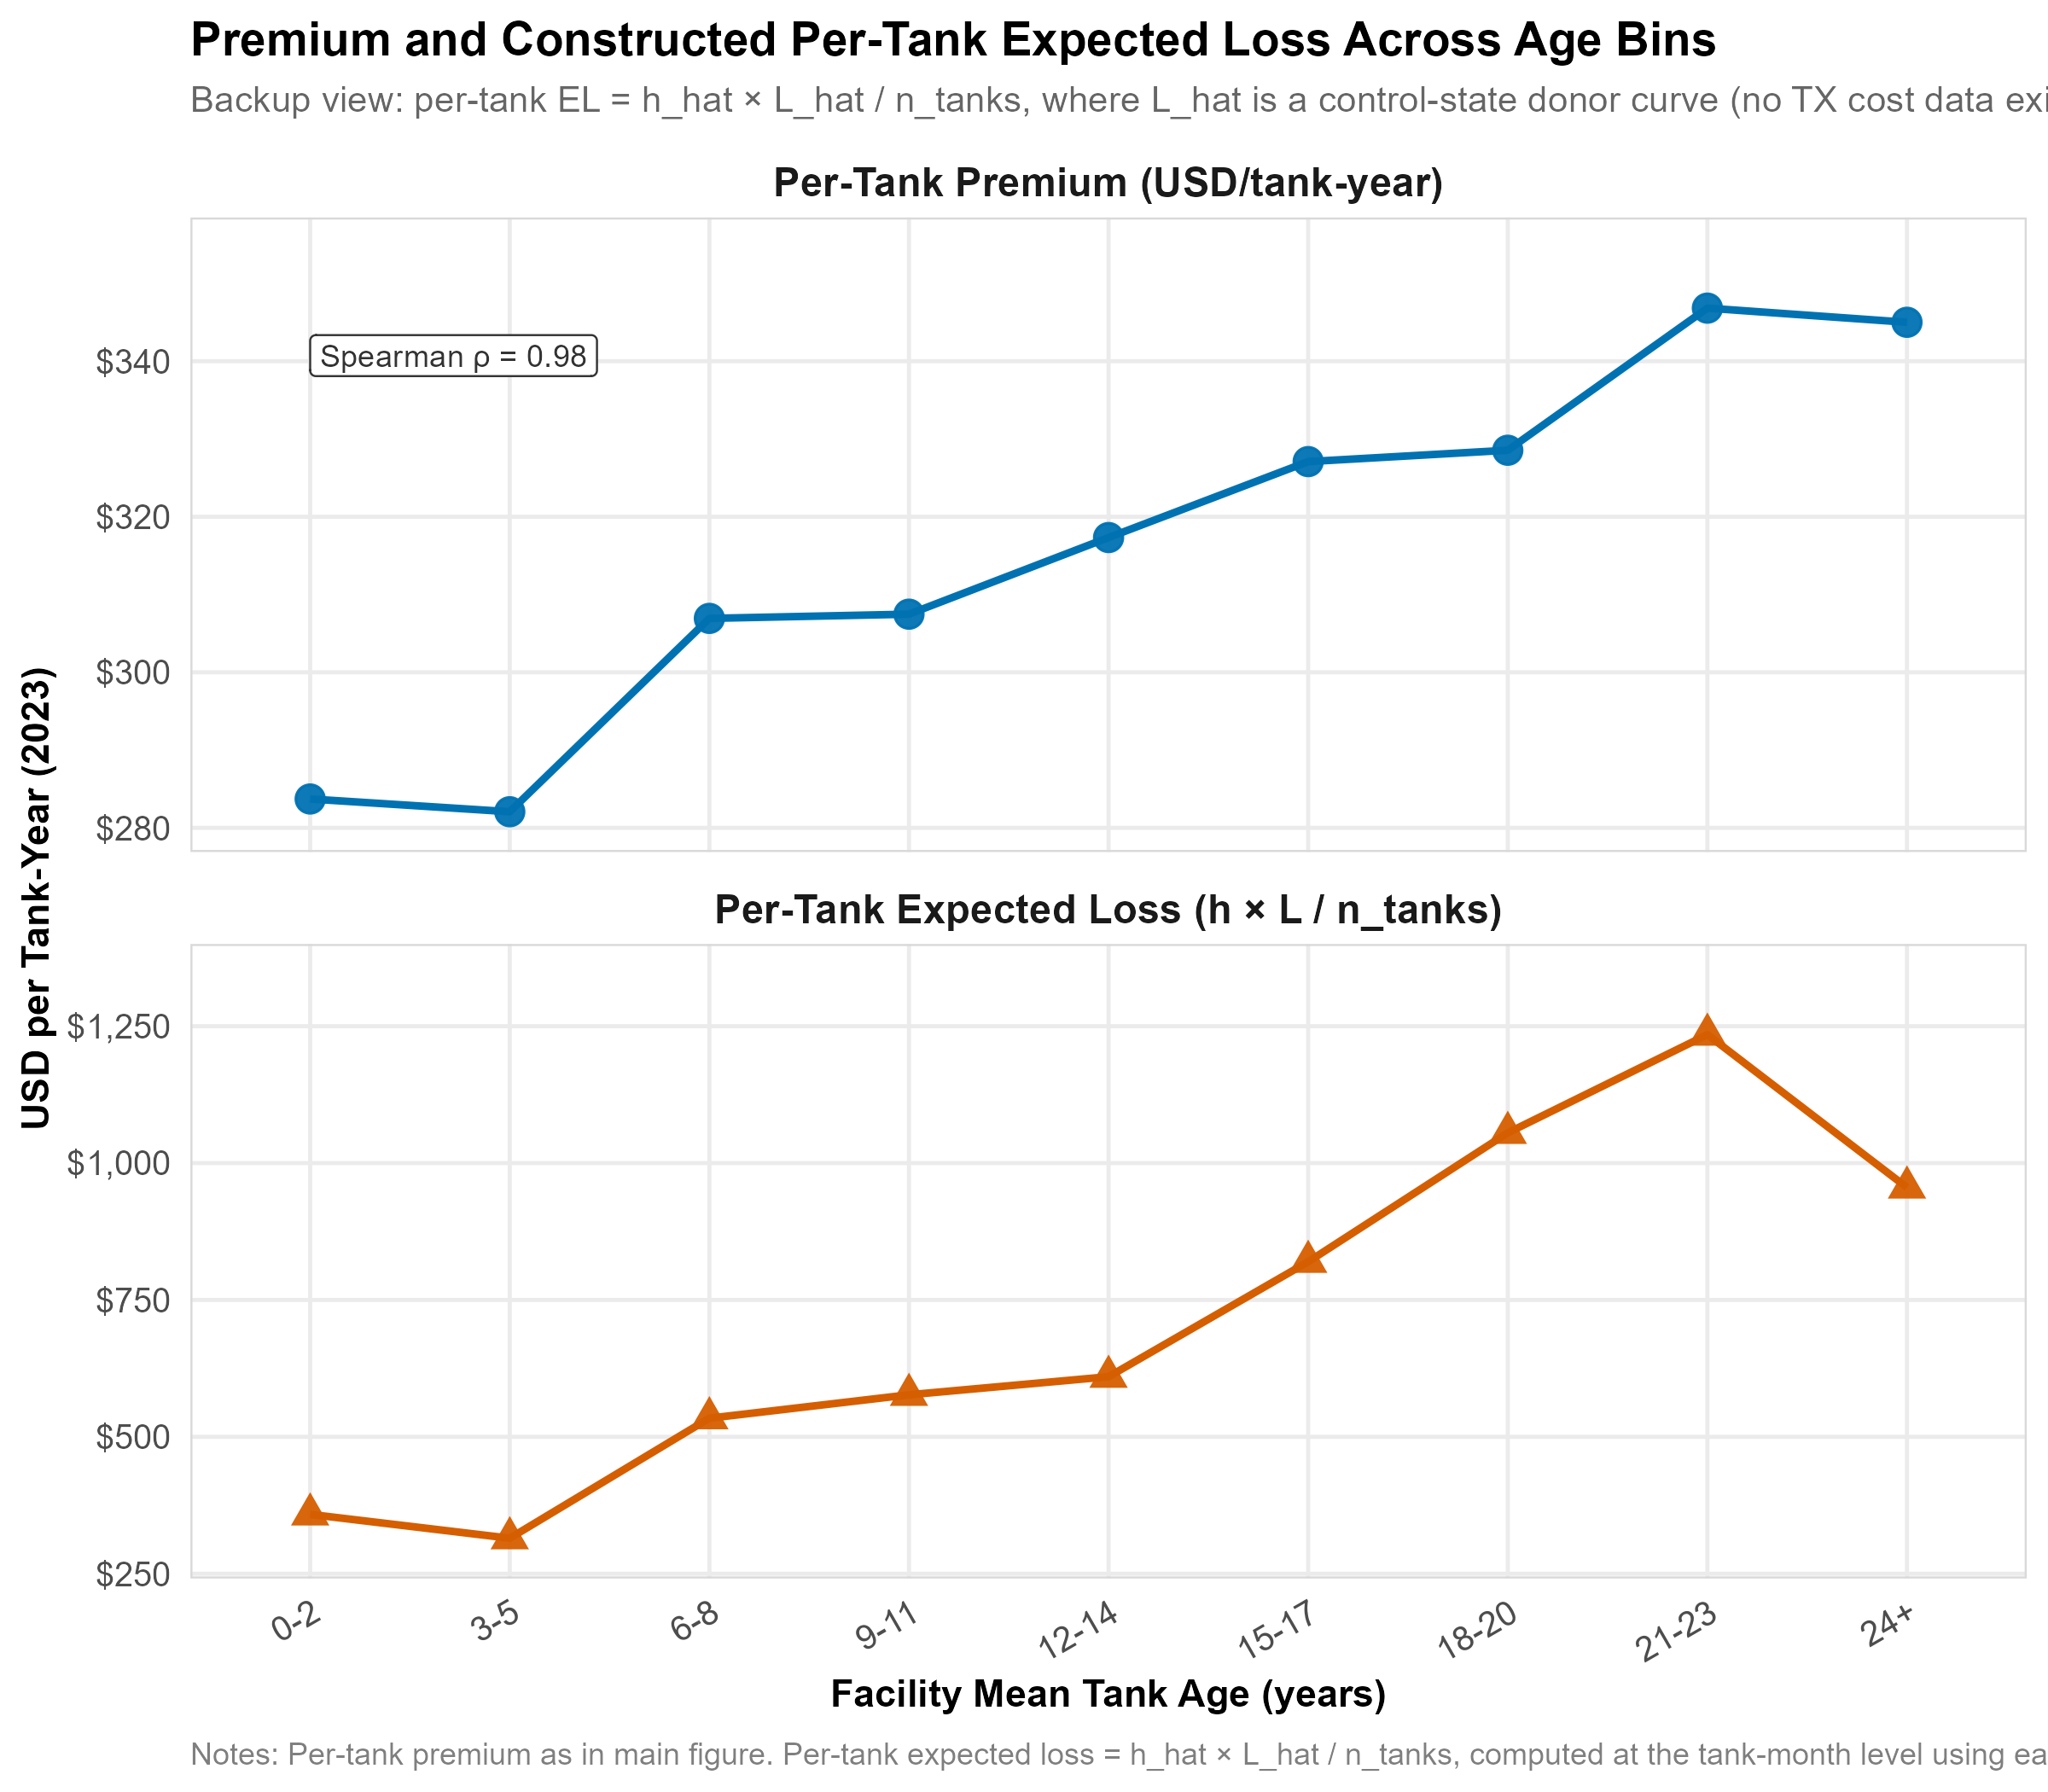
\includegraphics[width=0.92\textwidth,height=0.78\textheight,keepaspectratio]{../../Output/Figures/Figure_Premium_vs_EL_Raw.png}
\end{center}

\begin{tikzpicture}[remember picture, overlay]
\node[anchor=south west, inner sep=0pt] at ([xshift=10pt, yshift=10pt]current page.south west) {%
  \navbutton[slide-data][fill=BerkeleyBlue, font=\tiny, inner sep=2pt]{$\leftarrow$ back}%
};
\end{tikzpicture}
\end{frame}

\begin{frame}{Appendix: Facility size at reform --- Texas vs.~controls}
\phantomsection\label{appendix-facility-size-at-reform-texas-vs.-controls}
\BerkeleyLightMode

\hypertarget{baseline-tanks}{}

\vspace{0.2cm}
\begin{center}
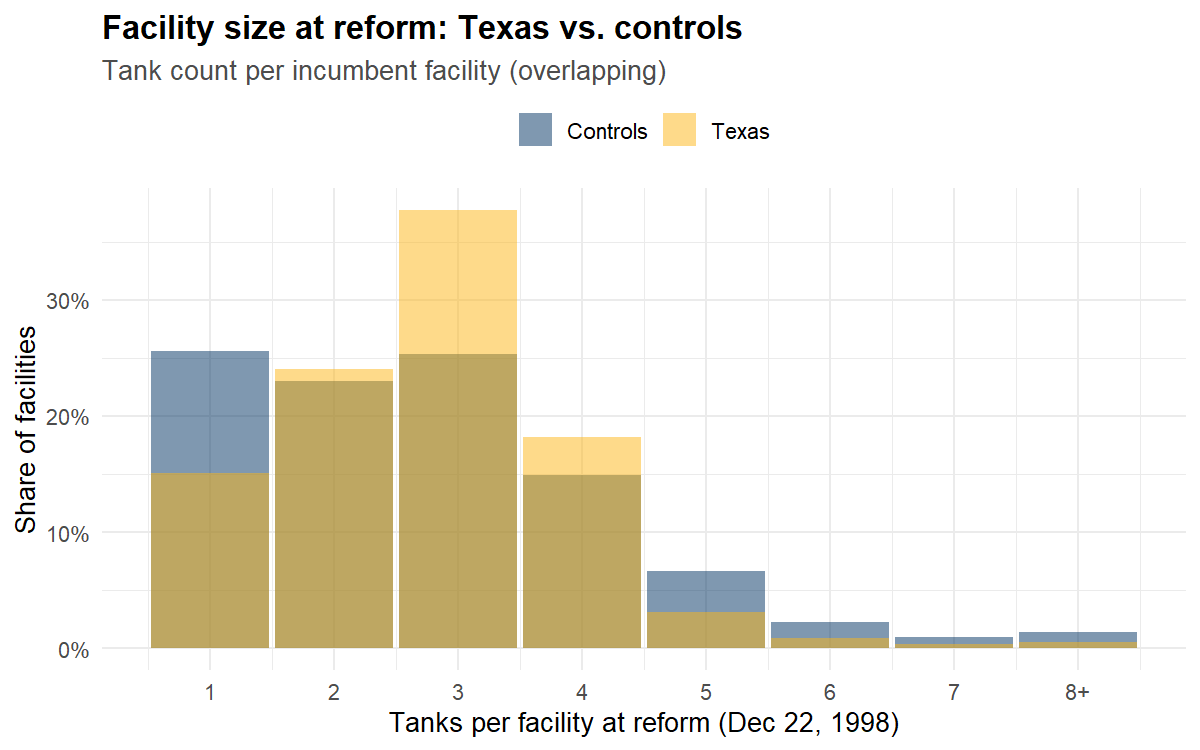
\includegraphics[width=0.92\textwidth,height=0.78\textheight,keepaspectratio]{../../Output/Figures/Fig_Baseline_TanksAtReform.png}
\end{center}

\begin{tikzpicture}[remember picture, overlay]
\node[anchor=south west, inner sep=0pt] at ([xshift=10pt, yshift=10pt]current page.south west) {%
  \navbutton[baseline-table][fill=BerkeleyBlue, font=\tiny, inner sep=2pt]{$\leftarrow$ back}%
  \hspace{3pt}%
  \navbutton[baseline-cap][fill=BerkeleyBlue, font=\tiny, inner sep=2pt]{Capacity $\rightarrow$}%
};
\end{tikzpicture}
\end{frame}

\begin{frame}{Appendix: Facility capacity at reform --- Texas
vs.~controls}
\phantomsection\label{appendix-facility-capacity-at-reform-texas-vs.-controls}
\BerkeleyLightMode

\hypertarget{baseline-cap}{}

\vspace{0.2cm}
\begin{center}
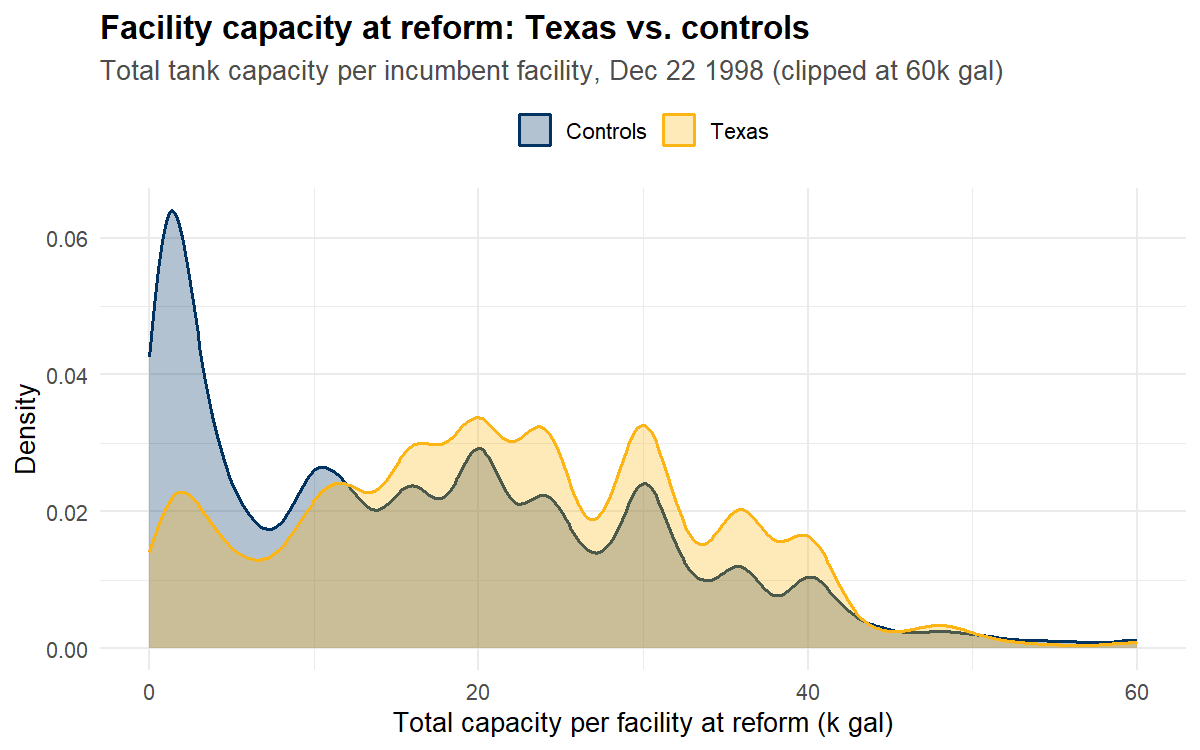
\includegraphics[width=0.92\textwidth,height=0.78\textheight,keepaspectratio]{../../Output/Figures/Fig_Baseline_CapacityAtReform.png}
\end{center}

\begin{tikzpicture}[remember picture, overlay]
\node[anchor=south west, inner sep=0pt] at ([xshift=10pt, yshift=10pt]current page.south west) {%
  \navbutton[baseline-table][fill=BerkeleyBlue, font=\tiny, inner sep=2pt]{$\leftarrow$ back}%
};
\end{tikzpicture}
\end{frame}

\begin{frame}{Appendix: How the model codes each facility-year}
\phantomsection\label{appendix-how-the-model-codes-each-facility-year}
\BerkeleyLightMode

\hypertarget{model-coding}{}

Let \(k_{it}\) = tanks closed and \(m_{it}\) = tanks installed in year
\(t\). Each facility-year gets exactly one action, by precedence:

\begin{align*}
\textbf{Exit } X         &: \quad \text{every tank closed} \\
\textbf{Replace } (k,m\ge 1) &: \quad k_{it}\ge 1,\;\; m_{it}\ge 1,\;\; \text{still operating} \\
\textbf{Downsize } (k,0) &: \quad k_{it}\ge 1,\;\; m_{it}=0,\;\; \text{still operating} \\
\textbf{Maintain } (0,0) &: \quad k_{it}=0
\end{align*}

\vspace{0.1cm}

\begin{itemize}
\tightlist
\item
  \textbf{State} coded from the beginning-of-year portfolio: counts
  \(n\) over 16 (wall \(\times\) age) cells, capacity bin \(G\), regime
  \(\rho\)
\item
  \textbf{Which tanks leave} is the rule \(r(n,k)\) --- oldest
  single-walled first --- \emph{not} a choice; only the counts \(k,\,m\)
  are chosen
\item
  The new tank enters double-walled at age bin 1 (regulation)
\end{itemize}

\vfill

\centering\small\textit{Downsizing --- coded ``maintain'' or ``exit'' in the single-tank model --- is now its own action.}

\begin{tikzpicture}[remember picture, overlay]
\node[anchor=south west, inner sep=0pt] at ([xshift=10pt, yshift=10pt]current page.south west) {%
  \navbutton[slide-structural][fill=BerkeleyBlue, font=\tiny, inner sep=2pt]{$\leftarrow$ back}%
};
\end{tikzpicture}
\end{frame}

\begin{frame}{Texas was first. The state-run uniform-premium model is
winding down nationwide}
\phantomsection\label{texas-was-first.-the-state-run-uniform-premium-model-is-winding-down-nationwide}
\BerkeleyLightMode

\begin{itemize}
\tightlist
\item
  Six states have already replaced their state-run uniform premium with
  private, risk-rated coverage: Arizona, Connecticut, Florida, New York,
  Texas, Wisconsin.
\item
  More than a dozen others carry a statutory fund sunset (claims-bar)
  date. The dates cluster through this decade:
\end{itemize}

\vspace{0.15cm}
\begin{center}
\small
Minnesota 2022 \quad Colorado 2023 \quad Kansas / Nebraska 2024 \\[3pt]
Illinois / New Hampshire / Missouri 2025 \quad California / South Carolina 2026 \\[3pt]
Utah 2028 \quad Vermont 2029 \quad Washington 2030 \quad Oklahoma 2032
\end{center}
\vspace{0.1cm}

\begin{itemize}
\tightlist
\item
  The gasoline fees that bankroll these programs are in structural
  decline as fuel use shifts (ASTSWMO 2023).
\end{itemize}

\vfill

\centering\small\textit{This paper measures the welfare consequences of exactly the transition many states are now facing. (California's 2026 date was pushed to 2036 in 2024, so these sunsets get re-litigated.) Source: ASTSWMO State Fund Survey.}
\end{frame}

\end{document}
